\documentclass[12pt,a4paper]{article}
\usepackage{caption}
\usepackage{float}
\usepackage{fontspec}
\setmainfont{Times New Roman}
\renewcommand{\figurename}{Hình}
\renewcommand{\tablename}{Bảng}
\usepackage{tocloft,calc}
\usepackage[top=3.5cm, bottom=3.0cm, left=3.5cm, right=2.0cm]{geometry} % căn lề theo quy chuẩn KLTN
\usepackage{amsmath,latexsym,amscd,amsfonts,mathrsfs,enumerate} \usepackage{ upgreek }
\usepackage[thref,thmmarks,standard,amsmath,hyperref]{ntheorem}
\usepackage[mathscr]{eucal}
\usepackage[unicode,colorlinks=true, bookmarks=true, pdfstartview=FitH,]{hyperref} %pagebackref=true,
\hypersetup{
pdftitle={Ứng dụng học tăng cường trong trò chơi Pacman},
pdfauthor={Đặng Anh Tuyền},
colorlinks = true,
linkcolor = black,
citecolor = blue,
urlcolor = blue,
}
\usepackage{fancyhdr}
\usepackage{graphicx}
\usepackage{fancybox,cite}
\usepackage{subcaption}
%\usepackage{refcheck}
 
\allowdisplaybreaks
%Môi trường định nghĩa
\theoremheaderfont{\bfseries} % In ra chữ "định nghĩa": đậm, thẳng đứng.
\theorembodyfont{} % Nội dung của định nghia được viết bằng chữ thẳng đứng.
\theoremseparator {}         % Ngăn cách giữa định nghĩa và nội dung định nghĩa bởi dấu chấm.
\newtheorem{dn}{Định nghĩa}[section] % Lệnh này để trong file kết quả in ra chữ nhận xét thay vì nếu ta để mặc định.

%Môi trường Ví dụ
\theoremheaderfont{\bfseries} % In ra chữ "Ví dụ": đậm, thẳng đứng.
\theorembodyfont{\normalfont} % Nội dung của ví dụ được viết bằng chữ thẳng đứng.
\theoremseparator {.}         % Ngăn cách giữa Ví dụ và nội dung ví dụ bởi dấu chấm.
\newtheorem{vd}{Ví dụ}[section] % Lệnh này để trong file kết quả in ra chữ Ví dụ thay vì Example nếu ta để mặc định.

%Môi trường Chú ý
\theoremstyle{plain} %Không đánh sỗ chú ý
\theoremheaderfont{\bfseries} % In ra chữ "chú ý": đậm, thẳng đứng.
\theorembodyfont{\normalfont} % Nội dung của chú ý được viết bằng chữ thẳng đứng.
\theoremseparator {}         % Ngăn cách giữa "chú ý" và nội dung chú ý bởi dấu chấm.
\newtheorem{cy}{Chú ý} % Lệnh này để trong file kết quả in ra chữ "chú ý" thay vì remark nếu ta để mặc định.
\usepackage{booktabs}
\usepackage{tabularx}
\usepackage{multirow}
\usepackage{makecell}
\usepackage{tikz}
\usepackage{xurl}

\Urlmuskip=0mu plus 1mu
\emergencystretch=3em
\usetikzlibrary{arrows.meta,positioning,calc}

% Kiểu dùng chung cho các sơ đồ vector ở Chương 3.
\tikzset{
    chthreeflow/.style={-{Latex[length=2.5mm,width=1.7mm]}, line width=0.9pt, draw=blue!35!black, shorten <=2pt, shorten >=2pt},
    chthreedash/.style={-{Latex[length=2.3mm,width=1.5mm]}, line width=0.85pt, dashed, draw=blue!55!black, shorten <=2pt, shorten >=2pt},
    chthreeblue/.style={draw=blue!70!black, fill=blue!4, rounded corners=5pt, line width=0.8pt, align=center, inner sep=6pt},
    chthreegreen/.style={draw=green!55!black, fill=green!5, rounded corners=5pt, line width=0.8pt, align=center, inner sep=6pt},
    chthreepurple/.style={draw=violet!70!black, fill=violet!5, rounded corners=5pt, line width=0.8pt, align=center, inner sep=6pt},
    chthreeorange/.style={draw=orange!80!black, fill=orange!6, rounded corners=5pt, line width=0.8pt, align=center, inner sep=6pt}
}

% Hiển thị các số phương trình được dẫn lại bằng màu xanh.
\renewcommand{\eqref}[1]{%
    \hyperref[#1]{\textcolor{blue}{\textup{(\ref*{#1})}}}%
}

% Hiển thị số hình được dẫn lại bằng màu xanh, giữ chữ "Hình" màu đen.
\newcommand{\figref}[1]{%
    Hình~\hyperref[#1]{\textcolor{blue}{\ref*{#1}}}%
}

% Hiển thị số bảng được dẫn lại bằng màu xanh, giữ chữ "Bảng" màu đen.
\newcommand{\tabref}[1]{%
    Bảng~\hyperref[#1]{\textcolor{blue}{\ref*{#1}}}%
}

%Môi trường Bài tập
\theoremheaderfont{\bfseries} % In ra chữ "chú ý": đậm, thẳng đứng.
\theorembodyfont{\normalfont} % Nội dung của chú ý được viết bằng chữ thẳng đứng.
\theoremseparator {}         % Ngăn cách giữa "chú ý" và nội dung chú ý bởi dấu chấm.\newtheorem{bt}{Bài tập} % Lệnh này để trong file kết quả in ra chữ "chú ý" thay vì  remark nếu ta để mặc định.

%Môi trường nhân xét
\theoremheaderfont{\bfseries} % In ra chữ "Nhân xét": đậm, thẳng đứng.
\theorembodyfont{\normalfont} % Nội dung của nhạn xét được viết bằng chữ thẳng đứng.
\theoremseparator {}         % Ngăn cách giữa nhận xét và nội dung nhận xét bởi dấu chấm.
\newtheorem{nx}{Nhận xét}[section] % Lệnh này để trong file kết quả in ra chữ nhận xét thay vì nếu ta để mặc định.

%Môi trường định lý
\theoremstyle{plain} %Sử dụng phong cách plain để đánh số Định lý, chẳng hạn: Định lý 1, Định lý 2,...
\theoremheaderfont{\normalfont\bfseries} % In ra chữ "Định lý": đậm, thẳng đứng.
\theorembodyfont{\normalfont} % Nội dung của Định lý được viết bằng chữ nghiêng.
\theoremseparator {.}         % Ngăn cách giữa Định lý và nội dung định lý bởi dấu chấm.
\renewtheorem{theorem}{Định lý} % Lệnh này để trong file kết quả in ra chữ Định lý thay vì theorem nếu ta để mặc định.
%Môi trường Mệnh đề
\theoremstyle{plain} %Sử dụng phong cách plain để đánh số Mệnh đề, chẳng hạn: Mệnh đề 1, Mệnh đề 2,...
\theoremheaderfont{\normalfont\bfseries} % In ra chữ "Mệnh đề": đậm, thẳng đứng.
\theorembodyfont{\normalfont} % Nội dung của Mệnh đề được viết bằng chữ thẳng đứng.
\theoremseparator {.}         % Ngăn cách giữa Mệnh đề và nội dung mệnh đề bởi dấu chấm.
\renewtheorem{proposition}{Mệnh đề} % Lệnh này để trong file kết quả in ra chữ Mệnh đề thay vì proposition nếu ta để mặc định.
%Môi trường Chứng minh
\theoremstyle{nonumberplain}  % Kiểu định dạng dành cho chứng minh
\theoremheaderfont{\normalfont\bfseries} % Tiêu đề "Chứng minh" in nghiêng
\theorembodyfont{\normalfont}
\theoremseparator{.} 
\theoremsymbol{\ensuremath{\square}} % Dấu kết thúc chứng minh là ô vuông
\newtheorem{cm}{Chứng minh}[section]

\pagestyle{fancy}
\fancyhf{}
\fancyhead[L]{\itshape Nhập môn trí tuệ nhân tạo 2-3-25(N01)}
\fancyfoot[L]{\fontsize{9}{11}\selectfont\itshape Ứng dụng học tăng cường trong trò chơi Pacman}
\fancyfoot[C]{\thepage}
\setlength{\headheight}{16pt}
\renewcommand{\headrulewidth}{1.2pt}
\renewcommand{\footrulewidth}{1.2pt} % Cái này là tiêu đề chạy
\fancypagestyle{plain}{
    \fancyhf{}
    \fancyhead[L]{\itshape Nhập môn trí tuệ nhân tạo 2-3-25(N01)}
    \fancyfoot[L]{\fontsize{9}{11}\selectfont\itshape Ứng dụng học tăng cường trong trò chơi Pacman}
    \fancyfoot[C]{\thepage}
    \renewcommand{\headrulewidth}{1.2pt}
    \renewcommand{\footrulewidth}{1.2pt}
}

\numberwithin{equation}{section}
\numberwithin{figure}{section}
\numberwithin{table}{section}

\begin{document}
 \fontsize{14pt}{20pt}\selectfont % Lệnh thay đổi cỡ chữ thành cỡ 14, cỡ dòng 20 (theo quy chuẩn của Khóa Luận TN).
 \hypersetup{pageanchor=false}
 
 \thisfancypage{\setlength{\fboxsep}{0.2cm}\setlength{\fboxrule}{1pt}\doublebox}{}
 \begin{titlepage}
\begin{center}
	\large
	BỘ GIÁO DỤC VÀ ĐÀO TẠO\\
	\textbf{ĐẠI HỌC PHENIKAA}\\
	\textbf{TRƯỜNG CÔNG NGHỆ THÔNG TIN}\\[0.15cm]
	\rule{3.2cm}{0.4pt}\,o0o\,\rule{3.2cm}{0.4pt}
\end{center}
\vspace{-0.5cm}
\begin{center}
    
\includegraphics[scale=0.8]{image/Logo.png}\\[1cm] 
\end{center} 
\vspace{0.3 cm}
\begin{center}
    \bf\Large {BÁO CÁO BÀI TẬP LỚN}
\end{center}
\begin{center}
    \bf\large {HỌC PHẦN: NHẬP MÔN TRÍ TUỆ NHÂN TẠO 2-3-25(N01)}
\end{center}
\vspace{0.3 cm}
\begin{center}
	\bf\large ĐỀ TÀI: ỨNG DỤNG HỌC TĂNG CƯỜNG TRONG TRÒ CHƠI PACMAN
\end{center}
\begin{center}
	\normalsize
	\renewcommand{\arraystretch}{1.15}
	\begin{tabular}{@{}p{5.2cm}l@{}}
        \textbf{Đặng Anh Tuyền} & \textbf{MSSV:} 23010912 \\
                                & \textbf{Lớp:} K17-KHMT(AI\&KHDL)\_1 \\[0.25cm]
        \textbf{Nguyễn Thị Khánh Linh} & \textbf{MSSV:} 23016112 \\
                                        & \textbf{Lớp:} K17-KHMT(AI\&KHDL)\_1 \\[0.25cm]
        \textbf{Lý Thành Đạt} & \textbf{MSSV:} 23010879 \\
                               & \textbf{Lớp:} K17-KHMT(AI\&KHDL)\_1
	\end{tabular}
\end{center}

\vskip 0.8 cm
  \begin{center}
   GVHD: TS. Trần Đình Tân
  \end{center}
\vskip 0.5 cm
  \begin{center}
   {\large\textbf{Hà Nội, Tháng 8 năm 2026}}
  \end{center}
 \end{titlepage}

% Bìa lót: bố cục học thuật theo mẫu, có khung đôi và không sử dụng logo.
\begin{titlepage}
\thispagestyle{empty}
\thisfancypage{\setlength{\fboxsep}{0.2cm}\setlength{\fboxrule}{1pt}\doublebox}{}
\begin{center}
	\large
	BỘ GIÁO DỤC VÀ ĐÀO TẠO\\
	\textbf{ĐẠI HỌC PHENIKAA}\\
	\textbf{TRƯỜNG CÔNG NGHỆ THÔNG TIN}\\[0.15cm]
	\rule{4cm}{0.4pt}\,o0o\,\rule{4cm}{0.4pt}
\end{center}
\vspace{1.5cm}
\begin{center}
	\normalsize
	\renewcommand{\arraystretch}{1.15}
	\begin{tabular}{@{}p{5.2cm}l@{}}
        \textbf{Đặng Anh Tuyền} & \textbf{MSSV:} 23010912 \\
                                & \textbf{Lớp:} K17-KHMT(AI\&KHDL)\_1 \\[0.25cm]
        \textbf{Nguyễn Thị Khánh Linh} & \textbf{MSSV:} 23016112 \\
                                        & \textbf{Lớp:} K17-KHMT(AI\&KHDL)\_1 \\[0.25cm]
        \textbf{Lý Thành Đạt} & \textbf{MSSV:} 23010879 \\
                               & \textbf{Lớp:} K17-KHMT(AI\&KHDL)\_1
	\end{tabular}
\end{center}
\vspace{1.3cm}
\begin{center}
    \bf\Large {BÁO CÁO BÀI TẬP LỚN}
\end{center}
\begin{center}
    \bf\large {HỌC PHẦN: NHẬP MÔN TRÍ TUỆ NHÂN TẠO 2-3-25(N01)}
\end{center}
\vspace{0.65cm}
\begin{center}
	\bf\Large ỨNG DỤNG HỌC TĂNG CƯỜNG\\
    TRONG TRÒ CHƠI PACMAN
\end{center}
\vfill
\begin{center}
    GVHD: TS. Trần Đình Tân
\end{center}
\vfill
\begin{center}
    {\large\textbf{Hà Nội, Tháng 8 năm 2026}}
\end{center}
\vspace{0.25cm}
\end{titlepage}

% Bảng phân chia công việc của nhóm.
\begin{titlepage}
\thispagestyle{empty}
\begin{center}
    {\bfseries\Large BẢNG PHÂN CHIA CÔNG VIỆC}
\end{center}
\vspace{0.45cm}

\begingroup
\fontsize{10.5pt}{12.5pt}\selectfont
\setlength{\tabcolsep}{4pt}
\setlength{\arrayrulewidth}{0.7pt}
\renewcommand{\arraystretch}{1.08}
\begin{center}
\begin{tabularx}{\textwidth}{|
    >{\centering\arraybackslash}m{0.8cm}|
    >{\centering\arraybackslash}m{3.5cm}|
    >{\centering\arraybackslash}m{1.75cm}|
    >{\raggedright\arraybackslash}X|
    >{\centering\arraybackslash}m{1.45cm}|}
\hline
\textbf{STT} & \centering\textbf{Họ và tên} & \textbf{Vai trò} & \centering\textbf{Nội dung công việc} & \textbf{Tỷ lệ} \\
\hline
1 & \makecell[c]{Đặng Anh Tuyền} & \textbf{Trưởng nhóm} &
-- Lập kế hoạch, phân công và theo dõi tiến độ chung.\newline
-- Xây dựng, tích hợp môi trường Mini Pacman.\newline
-- Nghiên cứu nguyên lý hoạt động của thuật toán DDQN.\newline
-- Cài đặt và cấu hình Q-Learning, DQN, Double DQN.\newline
-- Tổ chức quy trình huấn luyện và đánh giá chín cấu hình.\newline
-- Tổng hợp, đối chiếu kết quả thực nghiệm.\newline
-- Biên tập, chuẩn hóa và hoàn thiện báo cáo.\newline
-- Xây dựng, tổng hợp và hoàn thiện slide thuyết trình. & \textbf{40\%} \\
\hline
2 & \makecell[c]{Nguyễn Thị Khánh\\Linh} & Thành viên &
-- Tìm hiểu cơ sở lý thuyết về học tăng cường.\newline
-- Nghiên cứu nguyên lý và công thức cập nhật Q-Learning.\newline
-- Viết nội dung lý thuyết, thu thập tài liệu tham khảo về Q-Learning.\newline
-- Phân tích và trình bày kết quả Q-Learning từ số liệu do trưởng nhóm cung cấp.\newline
-- Rà soát nội dung, chính tả và hình thức báo cáo.\newline
-- Chuẩn bị slide và thuyết trình phần Q-Learning. & \textbf{30\%} \\
\hline
3 & \makecell[c]{Lý Thành Đạt} & Thành viên &
-- Tìm hiểu cơ sở lý thuyết về mạng nơ-ron sâu.\newline
-- Nghiên cứu nguyên lý hoạt động của thuật toán DQN.\newline
-- Viết nội dung lý thuyết, chuẩn bị sơ đồ minh họa kiến trúc DQN.\newline
-- Phân tích và trình bày kết quả DQN từ số liệu do trưởng nhóm cung cấp.\newline
-- Rà soát nội dung, chính tả và hình thức báo cáo.\newline
-- Chuẩn bị slide và thuyết trình phần DQN. & \textbf{30\%} \\
\hline
\end{tabularx}
\end{center}
\endgroup

\vspace{0.55cm}
\begin{center}
    {\fontsize{13pt}{16pt}\selectfont
    \textbf{Repository dự án:}\quad
    \href{https://github.com/tuyenda2011/DRL-Pacman}{\texttt{github.com/tuyenda2011/DRL-Pacman}}}
\end{center}
\end{titlepage}

\pagestyle{fancy}
\pagenumbering{arabic}
\setcounter{page}{1}
\hypersetup{pageanchor=true,linkcolor=black}

% Chèn mục lục
\renewcommand{\contentsname}{Mục lục}
\tableofcontents

% Ngắt trang tại đây để chuyển Danh mục hình ảnh sang trang mới
\newpage 
%\clearpage % (Bạn cũng có thể dùng \clearpage thay cho \newpage)

% Chèn danh mục hình ảnh
\renewcommand{\listfigurename}{Danh mục hình ảnh}
\listoffigures

% Chèn danh mục bảng
\clearpage
\renewcommand{\listtablename}{Danh mục bảng}
\listoftables

% Ngắt trang để phần nội dung bài viết bắt đầu ở trang mới
\clearpage
\section{GIỚI THIỆU ĐỀ TÀI}

\subsection{Bối cảnh và lý do lựa chọn}

Trong trí tuệ nhân tạo (Artificial Intelligence -- AI), ra quyết định tuần tự là lớp bài toán trong đó hệ thống phải lựa chọn hành động dựa trên trạng thái hiện tại, đồng thời xem xét ảnh hưởng của quyết định đó đối với các trạng thái và kết quả về sau. Học tăng cường (Reinforcement Learning -- RL) là một hướng tiếp cận cho lớp bài toán này. Thay vì được cung cấp sẵn hành động đúng cho từng tình huống, tác tử (agent) tương tác với môi trường, nhận phần thưởng và điều chỉnh cách lựa chọn hành động nhằm tối đa hóa phần thưởng tích lũy \cite{SuttonBarto2018}.

Trên cơ sở đó, nhóm lựa chọn Pacman làm môi trường xây dựng và đánh giá các thuật toán học tăng cường \cite{BerkeleyPacman2024}. Luật chơi trực quan nhưng vẫn thể hiện rõ đặc điểm của một bài toán ra quyết định tuần tự. Tại mỗi bước, tác tử phải lựa chọn hướng di chuyển dựa trên vị trí hiện tại, các vật phẩm còn lại và sự xuất hiện của các mối nguy hiểm trong mê cung. Thay vì sử dụng nguyên trạng một môi trường có sẵn, nhóm trực tiếp thiết kế và cài đặt Mini Pacman với bản đồ, không gian trạng thái, không gian hành động, cơ chế phần thưởng và điều kiện kết thúc riêng cho đề tài. Nhờ đó, nhóm có thể kiểm soát các yếu tố ảnh hưởng đến quá trình học và theo dõi trực tiếp hành vi của tác tử.

Trên môi trường này, nhóm cài đặt Q-Learning, DQN và Double DQN trong cùng một ứng dụng. Q-Learning biểu diễn giá trị của các cặp trạng thái--hành động bằng Q-table \cite{WatkinsDayan1992}. DQN sử dụng mạng nơ-ron để xấp xỉ hàm giá trị hành động, kết hợp replay buffer và target network trong quá trình huấn luyện \cite{Mnih2013,Mnih2015}. Double DQN thay đổi cách xây dựng giá trị mục tiêu nhằm giảm xu hướng đánh giá quá cao (overestimation) của DQN \cite{VanHasselt2016}. Việc triển khai ba thuật toán giúp nhóm khảo sát sự khác biệt giữa phương pháp dạng bảng, phương pháp xấp xỉ bằng mạng nơ-ron và một cải tiến trực tiếp của DQN. Trong quá trình thực hiện đề tài, mã nguồn và các cấu hình được nhóm phát triển, quản lý trong repository DRL-Pacman trên GitHub. Kết quả thực nghiệm cũng được lưu trữ và công bố tại đây \cite{DRLPacmanGitHub}.

\subsection{Mục tiêu nghiên cứu}

Mục tiêu tổng quát của đề tài là xây dựng môi trường Mini Pacman, cài đặt và so sánh Q-Learning, DQN và Double DQN trong bài toán điều khiển tác tử chơi Pacman. Qua đó, nhóm xem xét mối liên hệ giữa nguyên lý của từng thuật toán, cách triển khai trong ứng dụng và kết quả quan sát được từ thực nghiệm.

\noindent Các mục tiêu cụ thể gồm:

\begin{itemize}
    \item Xây dựng môi trường Mini Pacman với không gian trạng thái, không gian hành động, cơ chế phần thưởng và điều kiện kết thúc phù hợp cho quá trình huấn luyện tác tử.
    \item Cài đặt Q-Learning, DQN và Double DQN theo các nguyên lý được trình bày trong những công trình nền tảng, đồng thời tổ chức cấu hình, huấn luyện, đánh giá và lưu mô hình cho từng thuật toán \cite{WatkinsDayan1992,Mnih2013,Mnih2015,VanHasselt2016}.
    \item Thực hiện chín cấu hình thí nghiệm, tương ứng với ba thuật toán và ba mức learning rate, trong cùng môi trường và quy trình đánh giá.
    \item Thu thập và so sánh kết quả bằng các chỉ số reward, completion rate, win rate và steps. Loss chỉ được sử dụng khi phân tích DQN và Double DQN.
    \item Xây dựng demo các tác tử sau huấn luyện, từ đó kết hợp quan sát định tính với kết quả định lượng để đánh giá ưu điểm, hạn chế của từng phương pháp và giới hạn của thực nghiệm.
\end{itemize}

\subsection{Đối tượng và phạm vi nghiên cứu}

Đối tượng nghiên cứu của đề tài là ba thuật toán RL dựa trên giá trị: Q-Learning dạng bảng, DQN và Double DQN. Báo cáo tập trung vào nguyên lý hoạt động, cách cài đặt, quá trình huấn luyện và kết quả thực nghiệm của ba thuật toán trong ứng dụng do nhóm xây dựng.

Thực nghiệm được tiến hành trên bản đồ \texttt{medium} có kích thước $15 \times 15$ ô của môi trường Mini Pacman. Tác tử Pacman lựa chọn một trong bốn hướng di chuyển và tương tác với thức ăn, viên sức mạnh, trái cây cùng ba con ma trong mê cung. Q-Learning sử dụng trạng thái rời rạc làm khóa của Q-table, trong khi DQN và Double DQN nhận vector đặc trưng được tạo từ trạng thái môi trường. Đề tài không nghiên cứu phương pháp học trực tiếp từ ảnh chụp màn hình.

Phạm vi thực nghiệm gồm chín cấu hình được tạo từ ba thuật toán và ba mức learning rate lựa chọn trước. Mỗi cấu hình được huấn luyện với một seed. Tại mỗi thời điểm đánh giá định kỳ, mô hình được chạy trong 20 lượt chơi (episode). Kết quả được xem xét qua reward, completion rate, win rate, steps và loss đối với các thuật toán sử dụng mạng nơ-ron. Đề tài chỉ khảo sát một bản đồ và không thực hiện tìm kiếm siêu tham số trên quy mô lớn. Vì vậy, các kết luận được giới hạn trong môi trường và cấu hình thực nghiệm của đề tài, không được xem là kết luận chung về hiệu quả của các thuật toán trong mọi bài toán.

\subsection{Đóng góp của đề tài}

Đóng góp chính của đề tài là xây dựng được môi trường Mini Pacman phục vụ quá trình huấn luyện và đánh giá tác tử RL. Môi trường mô phỏng mê cung, thức ăn, viên sức mạnh, trái cây, ba con ma, số mạng và các điều kiện kết thúc lượt chơi. Trên môi trường này, nhóm cài đặt Q-Learning, DQN và Double DQN trong cùng một ứng dụng, đồng thời xây dựng hệ thống cấu hình YAML, lưu checkpoint, lưu mô hình sau huấn luyện và đánh giá định kỳ.

Từ hệ thống đã xây dựng, nhóm thực hiện chín cấu hình huấn luyện tương ứng với ba thuật toán và ba mức learning rate. Kết quả được tổng hợp qua reward, completion rate, win rate, steps và loss khi phù hợp, qua đó hỗ trợ đánh giá các thuật toán từ nhiều khía cạnh. Bên cạnh các kết quả định lượng, nhóm còn xây dựng biểu đồ so sánh và demo các tác tử sau huấn luyện để quan sát trực tiếp hành vi của mô hình trong môi trường trò chơi.

\clearpage
\section{CƠ SỞ LÝ THUYẾT}

\subsection{Tổng quan về học tăng cường}

Học tăng cường (reinforcement learning -- RL) nghiên cứu cách một tác tử lựa chọn hành động khi tương tác với môi trường để tối đa hóa phần thưởng tích lũy. Khác với học có giám sát, tác tử không nhận sẵn nhãn cho từng quyết định. Thay vào đó, tác tử quan sát kết quả của các hành động đã thực hiện và điều chỉnh cách ra quyết định dựa trên phần thưởng nhận được. Bốn thành phần cơ bản của một hệ thống RL gồm chính sách, tín hiệu phần thưởng, hàm giá trị và mô hình môi trường nếu mô hình đó được biết hoặc được học \cite{SuttonBarto2018,TranDinhTanAICourse}.

Trong phạm vi đề tài, ba thuật toán Q-Learning, DQN và Double DQN đều thuộc nhóm phương pháp dựa trên giá trị (value-based methods). Các phương pháp này học giá trị của hành động trong từng trạng thái, sau đó ưu tiên hành động có giá trị ước lượng lớn nhất. Điểm khác biệt chính nằm ở cách biểu diễn giá trị hành động và cách xây dựng giá trị mục tiêu trong quá trình cập nhật.

\subsubsection{Quá trình quyết định Markov}

Quá trình quyết định Markov (Markov Decision Process -- MDP) là mô hình toán học cho bài toán ra quyết định tuần tự. Tại thời điểm $t$, tác tử nhận trạng thái $S_t \in \mathcal{S}$, lựa chọn hành động $A_t \in \mathcal{A}(S_t)$, sau đó môi trường trả về phần thưởng $R_{t+1}$ và trạng thái tiếp theo $S_{t+1}$. Chuỗi tương tác có dạng
\begin{equation}
    S_0, A_0, R_1, S_1, A_1, R_2, S_2, \ldots
    \label{eq:mdp-trajectory}
\end{equation}

Mối quan hệ giữa tác tử và môi trường được minh họa trong \figref{fig:agent-environment}. Hành động đi từ tác tử tới môi trường, còn trạng thái và phần thưởng đi theo chiều ngược lại.

\begin{figure}[H]
    \centering
    \begin{tikzpicture}[
        component/.style={
            draw,
            rounded corners=2pt,
            minimum width=4.0cm,
            minimum height=1.35cm,
            align=center,
            fill=black!4
        },
        flow/.style={-{Latex[length=2.5mm]}, thick}
    ]
        \node[component] (agent) {Tác tử};
        \node[component, right=5.0cm of agent] (environment) {Môi trường};

        \draw[flow]
            ([yshift=7pt]agent.east)
            --
            node[above]{Hành động $A_t$}
            ([yshift=7pt]environment.west);

        \draw[flow]
            ([yshift=-7pt]environment.west)
            --
            node[below, align=center]{Phần thưởng $R_{t+1}$\\Trạng thái $S_{t+1}$}
            ([yshift=-7pt]agent.east);
    \end{tikzpicture}
    \caption{Tương tác giữa tác tử và môi trường trong MDP \cite{SuttonBarto2018}.}
    \label{fig:agent-environment}
\end{figure}

Với MDP hữu hạn, động lực của môi trường có thể được mô tả bằng phân phối xác suất
\begin{equation}
    p(s',r \mid s,a)
    =
    \Pr\!\left\{
        S_{t+1}=s',\,R_{t+1}=r
        \mid
        S_t=s,\,A_t=a
    \right\}.
    \label{eq:mdp-dynamics}
\end{equation}
Phân phối này cho biết xác suất chuyển tới trạng thái $s'$ và nhận phần thưởng $r$ khi tác tử thực hiện hành động $a$ tại trạng thái $s$. Tính chất Markov yêu cầu trạng thái hiện tại phải chứa những thông tin từ quá khứ có ảnh hưởng đến diễn biến tương lai. Khi đã biết $S_t$ và $A_t$, xác suất của trạng thái cùng phần thưởng tiếp theo không phụ thuộc thêm vào toàn bộ lịch sử trước đó \cite{SuttonBarto2018}.

Một chính sách (policy) được ký hiệu bởi $\pi(a \mid s)$, biểu diễn xác suất lựa chọn hành động $a$ tại trạng thái $s$. Mục tiêu của tác tử là tìm chính sách tạo ra phần thưởng tích lũy kỳ vọng lớn. Đối với bài toán theo episode như Mini Pacman, mỗi episode kết thúc khi tác tử đạt điều kiện kết thúc của môi trường hoặc chạm giới hạn số bước.

\subsubsection{Phần thưởng tích lũy và hàm giá trị}

Phần thưởng tức thời chỉ phản ánh kết quả ngay sau một hành động. Để đánh giá ảnh hưởng dài hạn, RL sử dụng phần thưởng tích lũy có chiết khấu, còn gọi là return. Tại thời điểm $t$, return được định nghĩa là
\begin{equation}
    G_t
    =
    R_{t+1}
    + \gamma R_{t+2}
    + \gamma^2 R_{t+3}
    + \cdots
    =
    \sum_{k=0}^{\infty}\gamma^k R_{t+k+1},
    \label{eq:discounted-return}
\end{equation}
trong đó $\gamma \in [0,1]$ là discount factor. Giá trị $\gamma$ nhỏ làm tác tử ưu tiên phần thưởng gần, còn giá trị gần $1$ làm tăng ảnh hưởng của phần thưởng trong tương lai. Với bài toán theo episode, tổng trên kết thúc tại trạng thái terminal và giá trị sau thời điểm kết thúc được xem bằng $0$ \cite{SuttonBarto2018}.

Hàm giá trị trạng thái dưới chính sách $\pi$ được định nghĩa bởi
\begin{equation}
    v_{\pi}(s)
    =
    \mathbb{E}_{\pi}\!\left[G_t \mid S_t=s\right].
    \label{eq:state-value}
\end{equation}
Đại lượng này cho biết return kỳ vọng khi bắt đầu tại trạng thái $s$ và tiếp tục lựa chọn hành động theo $\pi$. Tương tự, hàm giá trị hành động là
\begin{equation}
    q_{\pi}(s,a)
    =
    \mathbb{E}_{\pi}\!\left[G_t \mid S_t=s, A_t=a\right],
    \label{eq:action-value}
\end{equation}
cho biết return kỳ vọng khi chọn hành động $a$ tại $s$, sau đó tiếp tục theo chính sách $\pi$.

Giá trị hành động tối ưu được ký hiệu là
\begin{equation}
    q_{*}(s,a)
    =
    \max_{\pi} q_{\pi}(s,a).
    \label{eq:optimal-action-value}
\end{equation}
Hàm này thỏa mãn phương trình tối ưu Bellman
\begin{equation}
    q_{*}(s,a)
    =
    \sum_{s',r}
    p(s',r \mid s,a)
    \left[
        r + \gamma \max_{a'} q_{*}(s',a')
    \right].
    \label{eq:bellman-optimality}
\end{equation}
Phương trình~\eqref{eq:bellman-optimality} là cơ sở của các thuật toán học giá trị. Giá trị của một cặp trạng thái--hành động được liên hệ với phần thưởng tức thời và giá trị tốt nhất có thể đạt được ở trạng thái tiếp theo \cite{SuttonBarto2018}.

\subsubsection{Khám phá và khai thác}

Trong quá trình học, tác tử phải cân bằng giữa khám phá (exploration) và khai thác (exploitation). Khai thác chọn hành động đang có Q-value lớn nhất, còn khám phá thử các hành động khác để thu thập thêm kinh nghiệm. Nếu chỉ khai thác từ đầu, tác tử có thể duy trì một hành động chưa thực sự tối ưu do các Q-value ban đầu còn thiếu chính xác. Nếu khám phá quá nhiều, tác tử không tận dụng được những gì đã học.

Một chiến lược phổ biến là $\epsilon$-greedy. Giả sử tại trạng thái $s$ chỉ có một hành động tham lam
\begin{equation}
    a^{*}
    =
    \underset{a' \in \mathcal{A}(s)}{\arg\max}\,Q(s,a').
    \label{eq:greedy-action}
\end{equation}
Xác suất lựa chọn hành động được xác định bởi
\begin{equation}
    \pi_{\epsilon}(a \mid s)
    =
    \begin{cases}
        1-\epsilon+\dfrac{\epsilon}{|\mathcal{A}(s)|},
        & \text{nếu } a=a^{*},\\[6pt]
        \dfrac{\epsilon}{|\mathcal{A}(s)|},
        & \text{nếu } a\neq a^{*}.
    \end{cases}
    \label{eq:epsilon-greedy}
\end{equation}
Với xác suất $1-\epsilon$, tác tử chọn hành động tham lam. Với xác suất $\epsilon$, tác tử chọn ngẫu nhiên trong tập hành động, vì vậy hành động tham lam vẫn có thể được chọn trong nhánh ngẫu nhiên. Trong thực nghiệm, $\epsilon$ thường giảm dần để ưu tiên khám phá ở giai đoạn đầu và khai thác nhiều hơn khi các Q-value đã ổn định hơn \cite{SuttonBarto2018}.

\subsection{Q-Learning}

Q-Learning được sử dụng trong đề tài như một phương pháp học dạng bảng. Thuật toán lưu Q-value của từng cặp trạng thái--hành động trong Q-table và cập nhật giá trị này từ phần thưởng cùng giá trị tốt nhất tại trạng thái tiếp theo. Q-Learning là phương pháp temporal-difference control không cần mô hình môi trường và thuộc nhóm off-policy: hành động tạo dữ liệu có thể được chọn bằng $\epsilon$-greedy, trong khi target sử dụng hành động có Q-value lớn nhất \cite{WatkinsDayan1992,SuttonBarto2018}.

Sau khi tác tử thực hiện $A_t$ tại $S_t$, nhận $R_{t+1}$ và chuyển tới $S_{t+1}$, phần tử tương ứng trong Q-table được cập nhật theo
\begin{equation}
    \begin{aligned}
    Q_{t+1}(S_t,A_t)
    =
    Q_t(S_t,A_t)
    + \alpha
    \Big[
        R_{t+1}
        + \gamma \max_{a'}Q_t(S_{t+1},a')
        - Q_t(S_t,A_t)
    \Big],
    \end{aligned}
    \label{eq:q-learning-update}
\end{equation}
trong đó $\alpha \in (0,1]$ là learning rate. Các phần tử khác của Q-table không thay đổi tại bước cập nhật này. Nếu $S_{t+1}$ là trạng thái terminal, thành phần giá trị tương lai được đặt bằng $0$.

Giá trị mục tiêu của cập nhật có thể viết là
\begin{equation}
    Y_t^{\mathrm{Q}}
    =
    R_{t+1}
    + \gamma \max_{a'}Q_t(S_{t+1},a'),
    \label{eq:q-learning-target}
\end{equation}
và sai số temporal difference là
\begin{equation}
    \delta_t
    =
    Y_t^{\mathrm{Q}}-Q_t(S_t,A_t).
    \label{eq:q-learning-td-error}
\end{equation}
Như vậy, Q-Learning dịch chuyển Q-value hiện tại một đoạn bằng $\alpha\delta_t$ về phía giá trị mục tiêu.

Quy trình của một bước Q-Learning gồm:
\begin{enumerate}
    \item Quan sát trạng thái hiện tại $S_t$.
    \item Chọn hành động $A_t$, thường bằng chiến lược $\epsilon$-greedy.
    \item Thực hiện hành động và nhận $R_{t+1}$ cùng $S_{t+1}$.
    \item Tính target theo phương trình~\eqref{eq:q-learning-target}.
    \item Cập nhật phần tử $Q(S_t,A_t)$ theo phương trình~\eqref{eq:q-learning-update}.
\end{enumerate}

Quy trình trên được minh họa trong \figref{fig:q-learning-principle}. Hình nhấn mạnh rằng mỗi bước chỉ cập nhật phần tử Q-value tương ứng với cặp trạng thái--hành động vừa quan sát.

\begin{figure}[H]
    \centering
    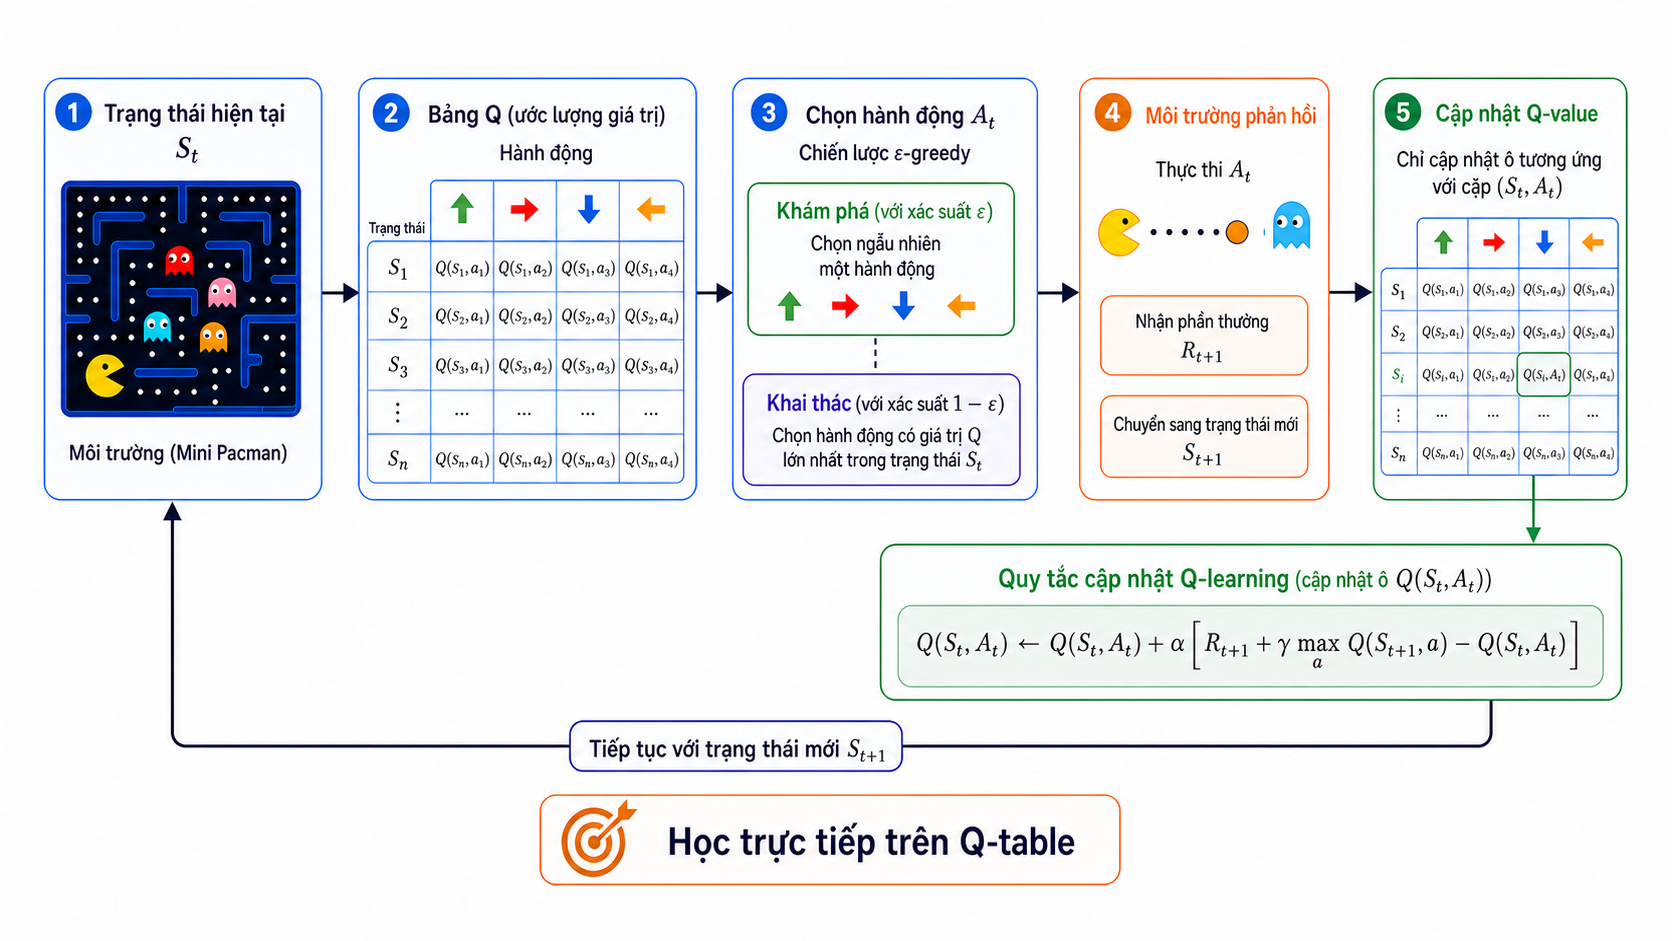
\includegraphics[width=\textwidth]{image/q_learning_principle.png}
    \caption{Quy trình lựa chọn hành động và cập nhật Q-table của Q-Learning \cite{WatkinsDayan1992,SuttonBarto2018}.}
    \label{fig:q-learning-principle}
\end{figure}

Về mặt lý thuyết, Q-Learning có thể hội tụ về action-value tối ưu với xác suất $1$ khi mọi cặp trạng thái--hành động tiếp tục được lấy mẫu và dãy learning rate thỏa mãn các điều kiện xấp xỉ ngẫu nhiên phù hợp \cite{WatkinsDayan1992}. Kết quả này không bảo đảm rằng mọi quá trình huấn luyện hữu hạn với learning rate cố định đều hội tụ.

Q-table giúp quy trình cập nhật dễ theo dõi nhưng phải lưu riêng Q-value cho từng cặp trạng thái--hành động. Khi số trạng thái tăng, kích thước bảng lớn hơn và các trạng thái khác nhau không có cơ chế chia sẻ thông tin. DQN xử lý hạn chế này bằng cách sử dụng mạng nơ-ron để xấp xỉ Q-value.

\subsection{Deep Q-Network}

Deep Q-Network (DQN) mở rộng Q-Learning bằng cách sử dụng mạng nơ-ron để xấp xỉ hàm giá trị hành động thay cho Q-table. Quá trình huấn luyện kết hợp experience replay nhằm tái sử dụng các chuyển tiếp và target network nhằm giữ giá trị mục tiêu ổn định hơn \cite{Mnih2013,Mnih2015}.

\subsubsection{Mạng Q}

Thay vì lưu một Q-table, DQN sử dụng mạng nơ-ron có tham số $\theta$ để xấp xỉ
\begin{equation}
    Q(s,a;\theta)
    \approx
    q_{*}(s,a).
    \label{eq:q-network-approximation}
\end{equation}
Với một trạng thái đầu vào, mạng Q xuất ra vector giá trị
\begin{equation}
    \mathbf{Q}(s;\theta)
    =
    \left[
        Q(s,a_1;\theta),
        Q(s,a_2;\theta),
        \ldots,
        Q(s,a_m;\theta)
    \right],
    \label{eq:q-network-output}
\end{equation}
trong đó $m$ là số hành động. Khi khai thác, tác tử chọn hành động có phần tử đầu ra lớn nhất. Trong quá trình khám phá, hành động vẫn được chọn theo chính sách $\epsilon$-greedy.

Q-network có thể nhận nhiều dạng biểu diễn trạng thái khác nhau. Trong đề tài, đầu vào của mạng là vector đặc trưng được xây dựng từ trạng thái Mini Pacman, không phải chuỗi khung hình như cấu hình Atari \cite{Mnih2013,Mnih2015}.

Do các trạng thái dùng chung tham số $\theta$, một lần cập nhật có thể làm thay đổi Q-value ước lượng của nhiều trạng thái. Điều này tạo khả năng khái quát hóa mà Q-table không có sẵn, nhưng cũng khiến target thay đổi trong quá trình học và có thể làm huấn luyện mất ổn định. DQN sử dụng experience replay và target network để giảm các vấn đề này.

\subsubsection{Experience replay}

Tại mỗi bước, tác tử thu được một chuyển tiếp
\begin{equation}
    e_t
    =
    (S_t,A_t,R_{t+1},S_{t+1}).
    \label{eq:transition}
\end{equation}
Các chuyển tiếp được lưu trong replay buffer $\mathcal{D}$. Khi cập nhật mạng, DQN không chỉ sử dụng chuyển tiếp mới nhất mà lấy ngẫu nhiên một mini-batch từ buffer. Với bài toán theo episode, cài đặt thực tế thường lưu thêm cờ kết thúc để xác định target có chứa giá trị tương lai hay không.

Experience replay có ba vai trò chính. Thứ nhất, một chuyển tiếp có thể được tái sử dụng trong nhiều lần cập nhật, giúp sử dụng dữ liệu hiệu quả hơn. Thứ hai, lấy mẫu ngẫu nhiên làm giảm tương quan mạnh giữa các chuyển tiếp liên tiếp. Thứ ba, dữ liệu trong buffer được tạo bởi nhiều phiên bản chính sách ở các thời điểm khác nhau, giúp làm mượt sự thay đổi của phân phối huấn luyện \cite{Mnih2013,Mnih2015}.

Replay buffer có dung lượng hữu hạn nên các chuyển tiếp cũ sẽ bị thay thế. Trong phạm vi đề tài, các chuyển tiếp được lấy mẫu đều từ buffer. Prioritized experience replay không được xem xét.

\subsubsection{Target network và loss}

DQN duy trì hai mạng có cùng kiến trúc:
\begin{itemize}
    \item Online network với tham số $\theta$ được cập nhật bằng gradient descent.
    \item Target network với tham số $\theta^{-}$ được dùng để tính giá trị mục tiêu.
\end{itemize}
Sau một số bước cập nhật cố định, tham số của online network được sao chép sang target network. Giữa hai lần đồng bộ, $\theta^{-}$ được giữ nguyên. Nhờ đó, target không thay đổi ngay sau từng lần cập nhật online network, làm giảm vòng phản hồi có thể gây dao động hoặc phân kỳ \cite{Mnih2015}.

Với một chuyển tiếp, target của DQN được xác định bởi
\begin{equation}
    Y_t^{\mathrm{DQN}}
    =
    \begin{cases}
        R_{t+1},
        & \text{nếu } S_{t+1} \text{ là terminal},\\[4pt]
        R_{t+1}
        + \gamma
        \displaystyle\max_{a'}
        Q(S_{t+1},a';\theta^{-}),
        & \text{trường hợp còn lại}.
    \end{cases}
    \label{eq:dqn-target}
\end{equation}
Online network tạo ra giá trị hiện tại $Q(S_t,A_t;\theta)$, còn target network tạo thành phần giá trị ở trạng thái tiếp theo.

Trong cài đặt của đề tài, online network được tối ưu bằng Smooth L1 Loss với ngưỡng chuyển tiếp bằng $1$. Gọi $\delta_i$ là TD error của mẫu thứ $i$, loss được xác định bởi
\begin{equation}
    \begin{aligned}
        \delta_i
        &=Y_i^{\mathrm{DQN}}-Q(s,a;\theta_i),\\
        L_i(\theta_i)
        &=\mathbb{E}_{(s,a,r,s')\sim U(\mathcal{D})}
        \left[\ell(\delta_i)\right],\\
        \ell(\delta)
        &=
        \begin{cases}
            \dfrac{1}{2}\delta^2, & \text{nếu } |\delta|<1,\\[4pt]
            |\delta|-\dfrac{1}{2}, & \text{trường hợp còn lại}.
        \end{cases}
    \end{aligned}
    \label{eq:dqn-loss}
\end{equation}
So với bình phương TD error, Smooth L1 Loss vẫn phạt sai lệch nhỏ theo dạng bậc hai nhưng chuyển sang dạng tuyến tính khi sai lệch lớn. Cách tính này đúng với hàm \texttt{SmoothL1Loss} được sử dụng trong mã nguồn của đề tài \cite{DRLPacmanGitHub}.
Learning rate của optimizer điều khiển độ lớn bước cập nhật tham số $\theta$ của online network khi tối ưu loss.

Luồng dữ liệu huấn luyện DQN được tổng hợp trong \figref{fig:dqn-training-flow}. Online network được cập nhật qua loss, còn target network chỉ nhận tham số qua bước đồng bộ định kỳ.

\begin{figure}[H]
    \centering
    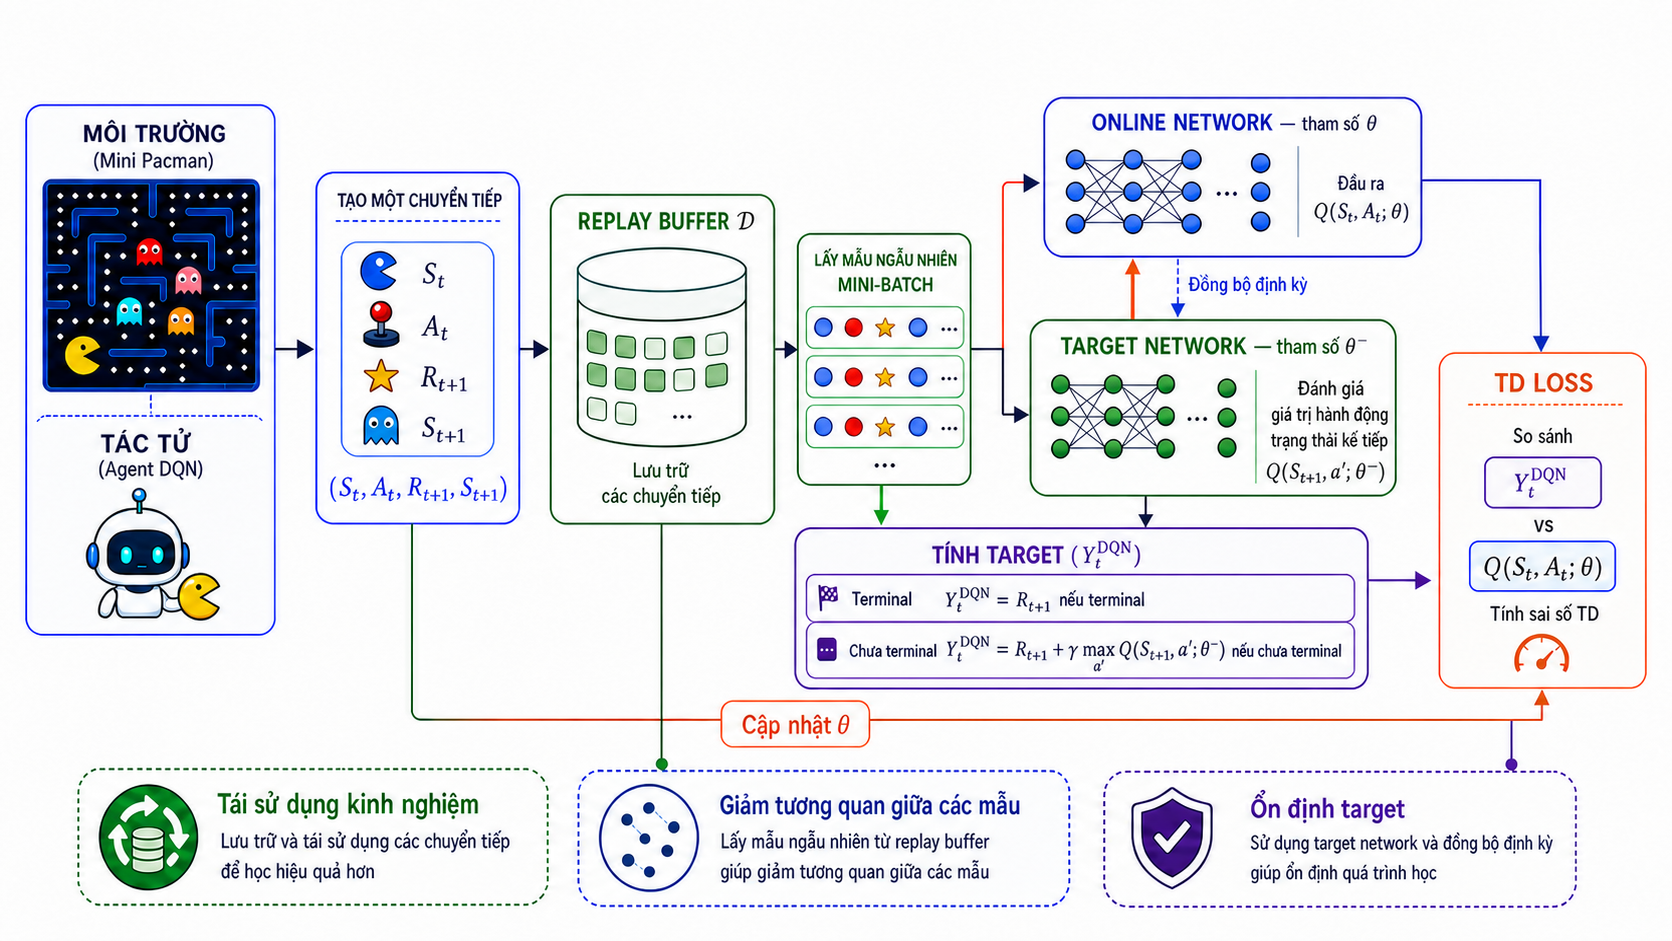
\includegraphics[width=\textwidth]{image/dqn_training_flow.png}
    \caption{Luồng huấn luyện DQN với experience replay và target network \cite{Mnih2013,Mnih2015}.}
    \label{fig:dqn-training-flow}
\end{figure}

\subsection{Double DQN}

Target của DQN trong phương trình~\eqref{eq:dqn-target} sử dụng cùng các giá trị do target network sinh ra để vừa chọn hành động có giá trị lớn nhất, vừa đánh giá hành động đó. Khi các Q-value chỉ là ước lượng và chứa sai số, phép lấy maximum có xu hướng ưu tiên những hành động đang bị đánh giá cao hơn giá trị thực. Hiện tượng này được gọi là overestimation \cite{VanHasselt2016}.

Đối với chuyển tiếp không kết thúc episode, target DQN có thể viết lại thành
\begin{equation}
    Y_t^{\mathrm{DQN}}
    =
    R_{t+1}
    +
    \gamma
    Q\!\left(
        S_{t+1},
        \underset{a'}{\arg\max}\,
        Q(S_{t+1},a';\theta_t^{-});
        \theta_t^{-}
    \right).
    \label{eq:dqn-target-expanded}
\end{equation}
Cả lựa chọn và đánh giá hành động đều dựa trên tham số $\theta_t^{-}$.

Double DQN tách hai vai trò này. Online network chọn hành động tham lam
\begin{equation}
    a_{t+1}^{*}
    =
    \underset{a'}{\arg\max}\,
    Q(S_{t+1},a';\theta_t),
    \label{eq:ddqn-action-selection}
\end{equation}
sau đó target network đánh giá hành động đã chọn. Target Double DQN là
\begin{equation}
    Y_t^{\mathrm{DDQN}}
    =
    \begin{cases}
        R_{t+1},
        & \text{nếu } S_{t+1} \text{ là terminal},\\[4pt]
        R_{t+1}
        + \gamma
        Q\!\left(
            S_{t+1},
            a_{t+1}^{*};
            \theta_t^{-}
        \right),
        & \text{trường hợp còn lại}.
    \end{cases}
    \label{eq:ddqn-target}
\end{equation}

Loss của Double DQN giữ nguyên dạng của phương trình~\eqref{eq:dqn-loss}, nhưng $Y_i^{\mathrm{DQN}}$ được thay bằng $Y_i^{\mathrm{DDQN}}$ khi tính TD error \cite{VanHasselt2016}.

Sự khác biệt nằm ở thành phần target. DQN lấy maximum trực tiếp từ target network, còn Double DQN dùng online network để chọn hành động và target network để đánh giá. Target network vẫn được đồng bộ định kỳ, còn optimizer và learning rate được giữ nguyên như DQN. Vì vậy, Double DQN không cần thêm mạng thứ ba và giữ nguyên phần còn lại của quy trình huấn luyện \cite{VanHasselt2016}.

Nguyên lý tách vai trò của Double DQN được minh họa trong \figref{fig:ddqn-selection-evaluation}. Online network chọn hành động tham lam tại trạng thái tiếp theo, còn target network đánh giá chính hành động đã chọn.

\begin{figure}[H]
    \centering
    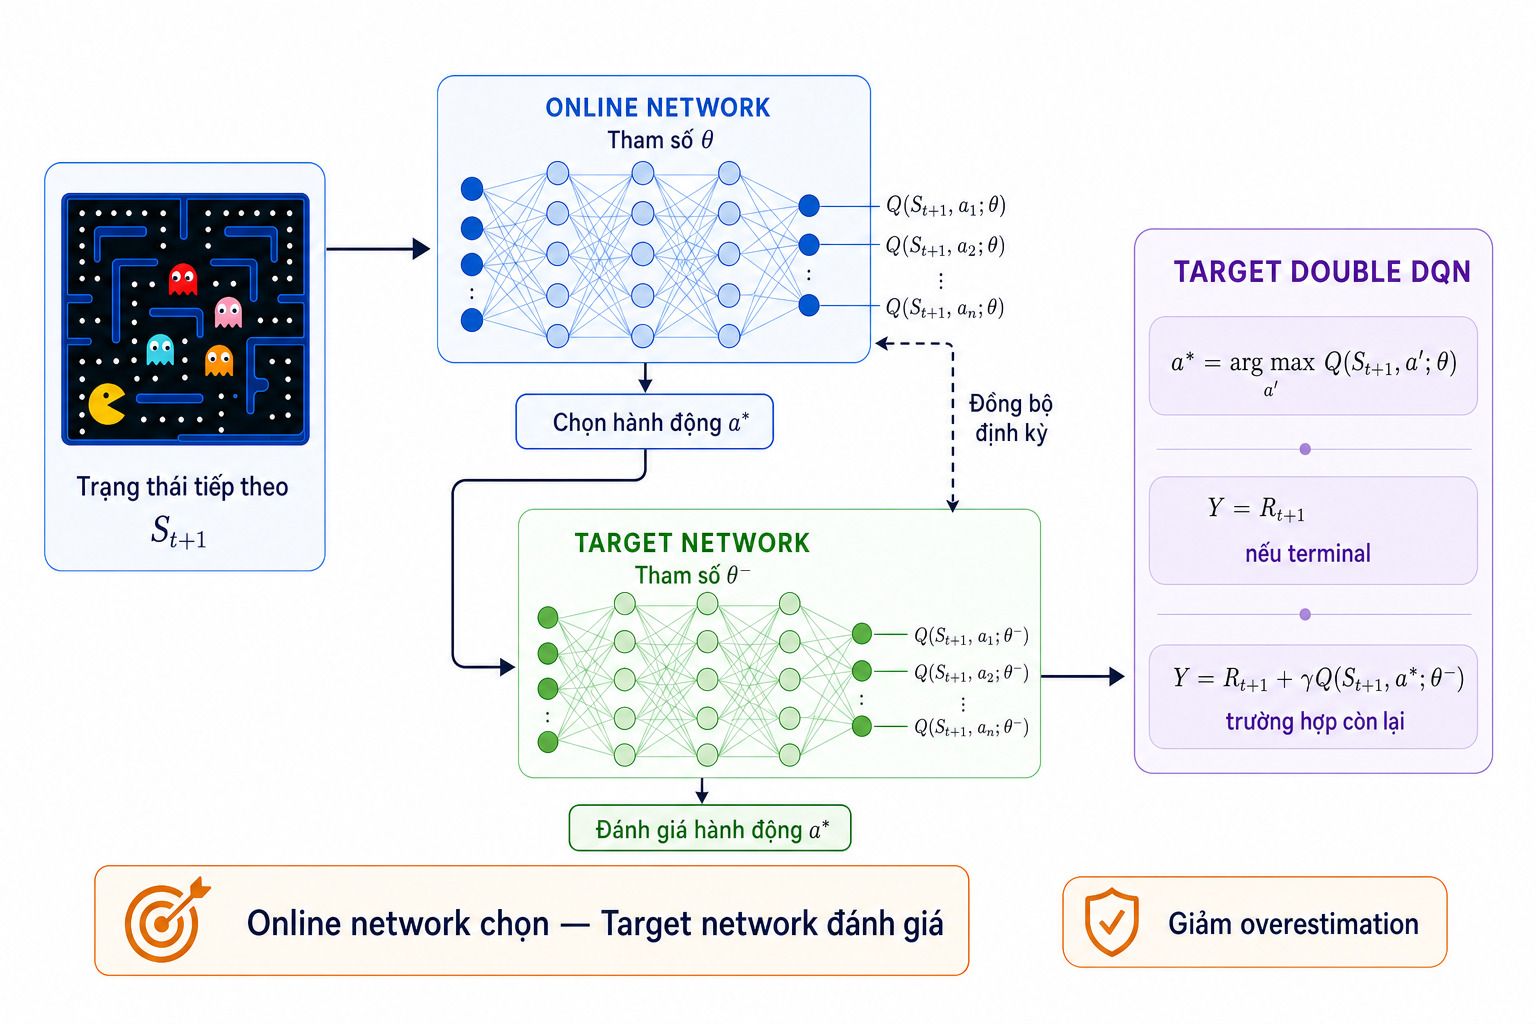
\includegraphics[width=\textwidth]{image/double_dqn_principle.png}
    \caption{Cơ chế lựa chọn và đánh giá hành động khi tính target Double DQN \cite{VanHasselt2016}.}
    \label{fig:ddqn-selection-evaluation}
\end{figure}

Double DQN làm giảm nhưng không loại bỏ hoàn toàn overestimation. Hiệu quả của cơ chế này vẫn phụ thuộc vào dữ liệu, biểu diễn trạng thái, kiến trúc mạng và cấu hình huấn luyện \cite{VanHasselt2016}.

\subsection{So sánh Q-Learning, DQN và Double DQN}

\tabref{tab:algorithm-theory-comparison} tổng hợp những khác biệt quan trọng về nguyên lý của ba thuật toán.

\begin{table}[H]
    \centering
    \renewcommand{\arraystretch}{1.25}
    \small
    \begin{tabular}{@{}
        >{\raggedright\arraybackslash}p{2.7cm}
        >{\raggedright\arraybackslash}p{3.5cm}
        >{\raggedright\arraybackslash}p{3.5cm}
        >{\raggedright\arraybackslash}p{3.5cm}
    @{}}
        \toprule
        \textbf{Tiêu chí} &
        \textbf{Q-Learning} &
        \textbf{DQN} &
        \textbf{Double DQN} \\
        \midrule
        Biểu diễn Q-value &
        Q-table với một phần tử cho mỗi cặp trạng thái--hành động. &
        Mạng Q có tham số $\theta$. &
        Online network và target network như DQN. \\

        Dữ liệu cập nhật &
        Cập nhật trực tiếp từ từng chuyển tiếp. &
        Mini-batch lấy ngẫu nhiên từ replay buffer. &
        Mini-batch lấy ngẫu nhiên từ replay buffer. \\

        Target ở trạng thái tiếp theo &
        Maximum của hàng Q-table tại trạng thái tiếp theo. &
        Target network vừa chọn vừa đánh giá hành động có giá trị lớn nhất. &
        Online network chọn hành động, target network đánh giá hành động đó. \\

        Khái quát hóa &
        Không có cơ chế chia sẻ giá trị giữa các trạng thái khác nhau. &
        Có khả năng chia sẻ thông tin thông qua tham số mạng. &
        Tương tự DQN. \\

        Loss của mạng nơ-ron &
        Không sử dụng. &
        Tối ưu TD error giữa Q-value hiện tại và target DQN. &
        Tối ưu TD error với target Double DQN. \\

        Hạn chế chính &
        Q-table tăng nhanh khi không gian trạng thái lớn. &
        Huấn luyện có thể mất ổn định và xuất hiện overestimation. &
        Giảm overestimation nhưng vẫn phụ thuộc vào hàm xấp xỉ và cấu hình huấn luyện. \\
        \bottomrule
    \end{tabular}
    \caption{So sánh Q-Learning, DQN và Double DQN về mặt nguyên lý.}
    \label{tab:algorithm-theory-comparison}
\end{table}

Q-Learning lưu trực tiếp Q-value trong Q-table. DQN sử dụng mạng nơ-ron để xấp xỉ Q-value, còn Double DQN giữ nguyên cơ chế huấn luyện của DQN nhưng tách quá trình lựa chọn và đánh giá hành động khi tính target.

Từ các cơ sở lý thuyết trên, chương tiếp theo trình bày cách nhóm cụ thể hóa bài toán Mini Pacman thành môi trường học tăng cường, bao gồm biểu diễn trạng thái, không gian hành động, cơ chế phần thưởng và điều kiện kết thúc. Trên nền tảng đó, Q-Learning, DQN và Double DQN được cài đặt trong cùng một hệ thống và đánh giá theo một quy trình thực nghiệm thống nhất.

\clearpage
\section{XÂY DỰNG HỆ THỐNG VÀ THIẾT KẾ THỰC NGHIỆM}

\subsection{Tổng quan ứng dụng học tăng cường trong trò chơi Pacman}

Đề tài xây dựng môi trường Mini Pacman để huấn luyện tác tử bằng ba phương pháp Q-Learning, DQN và Double DQN. Cả ba phương pháp cùng sử dụng một bản đồ, một bộ luật và một hệ tiêu chí đánh giá. Điểm khác biệt nằm ở cách biểu diễn và cập nhật hàm giá trị. Q-Learning lưu các Q-value trong Q-table, còn DQN và Double DQN xấp xỉ chúng bằng Q-network. Riêng DQN và Double DQN khác nhau ở cách xác định target cho bước cập nhật \cite{DRLPacmanGitHub}.

\figref{fig:system-overview} trình bày kiến trúc tổng thể của hệ thống. Trong mỗi bước tương tác, tác tử nhận state từ môi trường, chọn action rồi nhận reward, state kế tiếp và cờ kết thúc. Quá trình huấn luyện được điều khiển bởi cấu hình thực nghiệm và định kỳ lưu checkpoint cùng kết quả đánh giá. Khi huấn luyện kết thúc, mô hình cuối được dùng cho evaluation và demo mà không cập nhật thêm tham số.

\begin{figure}[H]
    \centering
    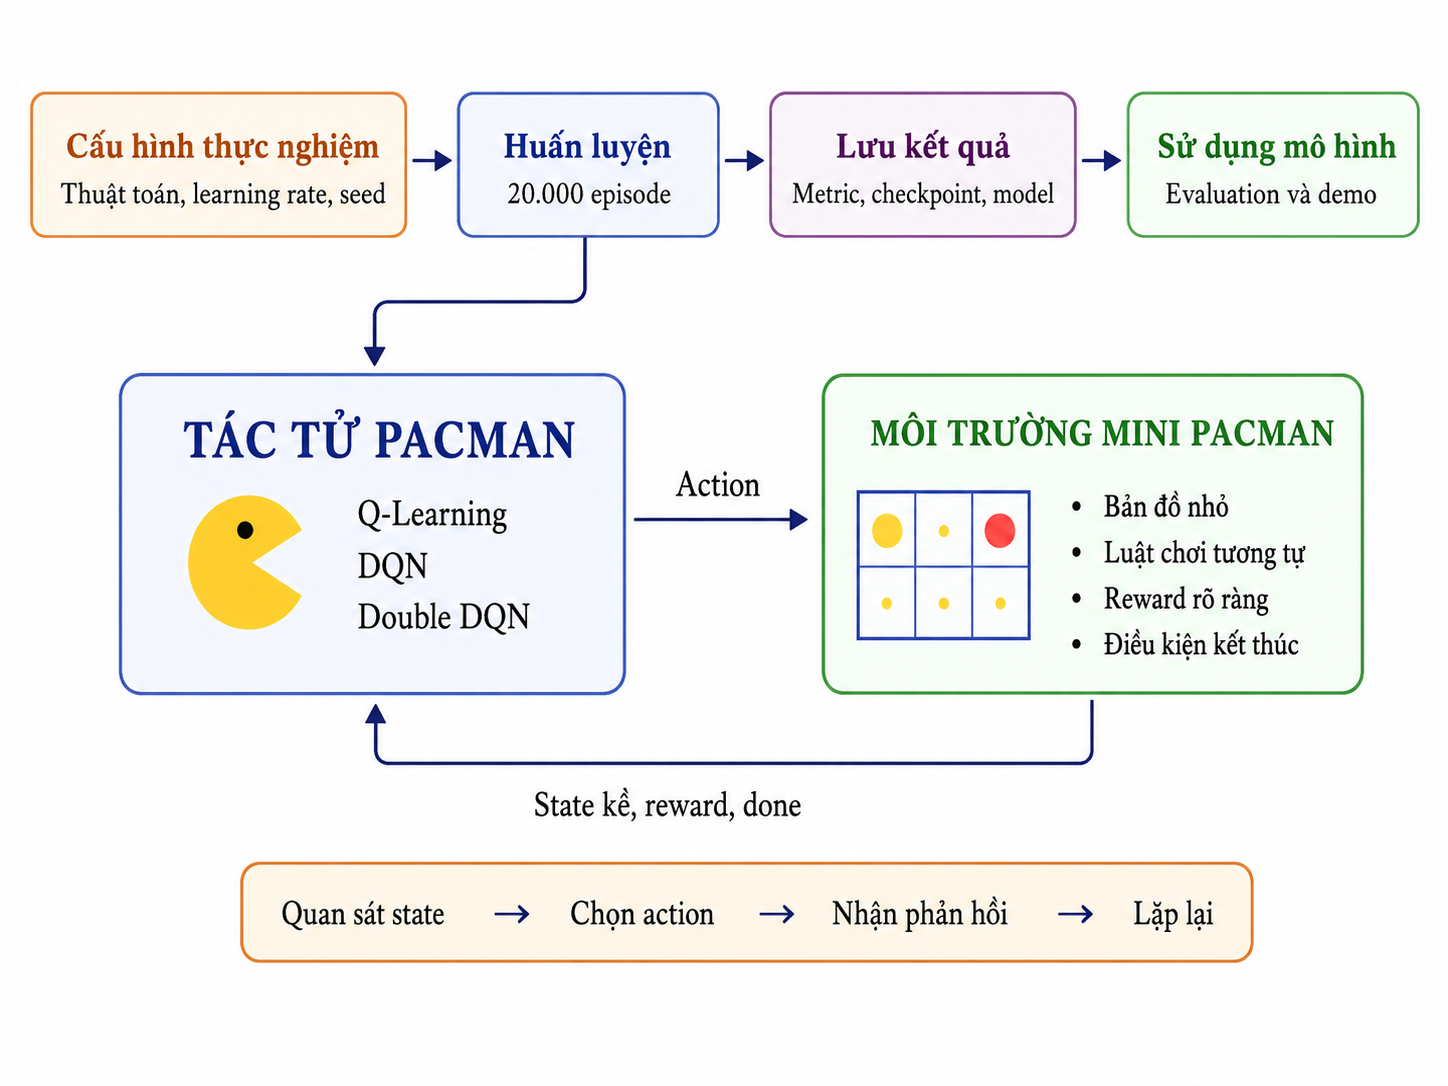
\includegraphics[width=0.94\textwidth]{image/hinh_3_1.png}
    \caption{Kiến trúc tổng thể của ứng dụng học tăng cường trong trò chơi Pacman.}
    \label{fig:system-overview}
\end{figure}

\subsection{Môi trường Mini Pacman}

Môi trường Mini Pacman tạo ra cùng một bài toán điều khiển cho cả ba phương pháp. Mỗi episode bắt đầu từ trạng thái khởi tạo của bản đồ. Sau khi nhận action, môi trường cập nhật trò chơi rồi trả về state kế tiếp, reward và cờ kết thúc. Tất cả thí nghiệm đều sử dụng bản đồ \texttt{medium}, ba mạng sống, ba ma và giới hạn 700 bước cho mỗi episode \cite{DRLPacmanGitHub}.

\subsubsection{Bản đồ và các thành phần trong môi trường}

Bản đồ \texttt{medium} có kích thước $15\times15$, gồm tường, hành lang, ghost door và khu vực xuất phát của ba ma ở trung tâm. Pacman xuất hiện ở phần dưới bản đồ. Hệ thống hành lang có nhiều ngã rẽ, buộc tác tử phải cân bằng giữa việc thu thập food, tránh ma và lựa chọn đường đi phù hợp.

Bản đồ chứa 62 food, trong đó bốn food gần các góc là power pellet. Ngoài ra, hai bonus fruit được đặt tại các vị trí cố định. Power pellet vẫn được tính vào tổng số food cần thu thập. Bonus fruit chỉ mang lại reward bổ sung và không ảnh hưởng đến điều kiện chiến thắng. \tabref{tab:map-components} tổng hợp các thành phần chính của môi trường.

\begin{table}[H]
    \centering
    \renewcommand{\arraystretch}{1.2}
    \small
    \begin{tabularx}{0.92\textwidth}{@{}
        >{\raggedright\arraybackslash}p{3.2cm}
        >{\centering\arraybackslash}p{2.1cm}
        >{\raggedright\arraybackslash}X
    @{}}
        \toprule
        \textbf{Thành phần} & \textbf{Số lượng} & \textbf{Vai trò trong môi trường} \\
        \midrule
        Bản đồ & $15\times15$ ô & Gồm tường, hành lang, ghost door và khu vực xuất phát của ma. \\
        Pacman & 1 & Tác tử được huấn luyện, bắt đầu với ba mạng sống. \\
        Ma & 3 & Blinky, Pinky và Inky, xuất phát tại khu vực trung tâm. \\
        Food & 62 & Phân bố trên hành lang và là điều kiện để hoàn thành bản đồ. \\
        Power pellet & 4 & Nằm trong 62 food và kích hoạt trạng thái frightened. \\
        Bonus fruit & 2 & Nằm ở vị trí cố định và cung cấp thêm reward. \\
        \bottomrule
    \end{tabularx}
    \caption{Các thành phần của bản đồ \texttt{medium} \cite{DRLPacmanGitHub}.}
    \label{tab:map-components}
\end{table}

\clearpage
\figref{fig:medium-map} minh họa trạng thái ban đầu của bản đồ trong một lượt demo. Bố cục bản đồ được giữ nguyên ở cả ba giai đoạn training, evaluation và demo.

\begin{figure}[H]
    \centering
    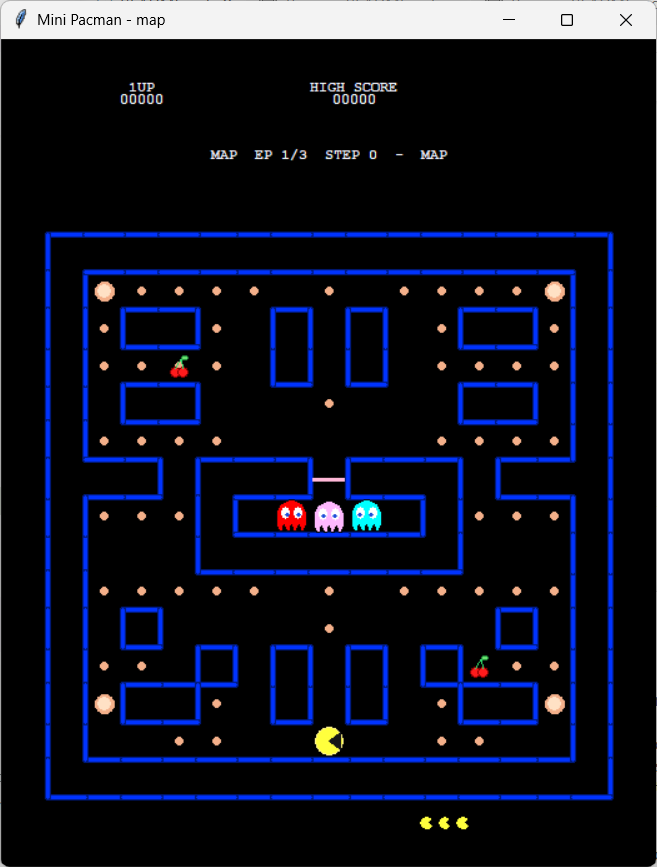
\includegraphics[width=0.49\textwidth]{image/demo_map.png}
    \caption{Bản đồ \texttt{medium} của môi trường Mini Pacman trong một lượt chạy demo.}
    \label{fig:medium-map}
\end{figure}

\subsubsection{Luật hoạt động và điều kiện kết thúc}

Trong mỗi environment step, Pacman di chuyển trước theo action đã chọn. Nếu hướng đi bị tường hoặc ghost door chặn, Pacman đứng tại chỗ và nhận penalty va tường. Sau đó, môi trường xử lý việc thu thập food, power pellet, bonus fruit và các va chạm tại vị trí mới. Ba ma tiếp tục thực hiện lượt di chuyển. Va chạm được kiểm tra thêm một lần trước khi môi trường trả về state mới, reward và cờ kết thúc.

Khi không frightened, ba ma luân phiên giữa scatter và chase. Mỗi ma sử dụng một mục tiêu riêng trong từng chế độ như trình bày trong \tabref{tab:ghost-targets}.

\begin{table}[H]
    \centering
    \renewcommand{\arraystretch}{1.14}
    \small
    \begin{tabularx}{0.96\textwidth}{@{}
        >{\raggedright\arraybackslash}p{2.5cm}
        >{\raggedright\arraybackslash}X
        >{\raggedright\arraybackslash}p{4.5cm}
    @{}}
        \toprule
        \textbf{Ma} &
        \makecell{\textbf{Mục tiêu trong}\\\textbf{chế độ chase}} &
        \makecell{\textbf{Mục tiêu trong}\\\textbf{chế độ scatter}} \\
        \midrule
        Blinky (đỏ) &
        Đuổi trực tiếp tới vị trí hiện tại của Pacman. &
        Góc trên bên phải của bản đồ, tại vị trí $(1,13)$. \\
        Pinky (hồng) &
        Nhắm tới điểm nằm trước Pacman tối đa bốn ô theo hướng di chuyển hiện tại để chặn đầu. &
        Góc trên bên trái của bản đồ, tại vị trí $(1,1)$. \\
        Inky (xanh lam) &
        Lấy điểm nằm trước Pacman tối đa hai ô, sau đó kéo dài vector từ Blinky tới điểm này thêm một lần để tạo mục tiêu. &
        Góc dưới bên phải của bản đồ, tại vị trí $(13,13)$. \\
        \bottomrule
    \end{tabularx}
    \caption{Mục tiêu di chuyển của ba ma trong chế độ chase và scatter \cite{DRLPacmanGitHub}.}
    \label{tab:ghost-targets}
\end{table}

Tại mỗi bước, ma loại hướng quay ngược nếu vẫn còn hướng hợp lệ khác, sau đó ưu tiên hướng tạo ra maze distance nhỏ nhất tới mục tiêu. Nếu nhiều hướng có cùng khoảng cách tốt nhất, hệ thống lựa chọn bằng bộ sinh số ngẫu nhiên đã được cố định seed. Cách xác định mục tiêu làm Blinky bám trực tiếp Pacman, Pinky tìm cách chặn đầu, còn Inky phối hợp vị trí của Blinky với hướng di chuyển của Pacman.

Power pellet đặt frightened timer bằng 35 bước. Trong thời gian này, ma chỉ di chuyển ở các environment step chẵn và ưu tiên hướng làm tăng maze distance tới Pacman. Nếu bị Pacman ăn, ma chuyển sang returning, quay về vị trí xuất phát rồi chờ bốn bước trước khi hoạt động trở lại. Các trạng thái chính và điều kiện chuyển đổi được minh họa trong \figref{fig:ghost-state-flow}.

\begin{figure}[H]
    \centering
    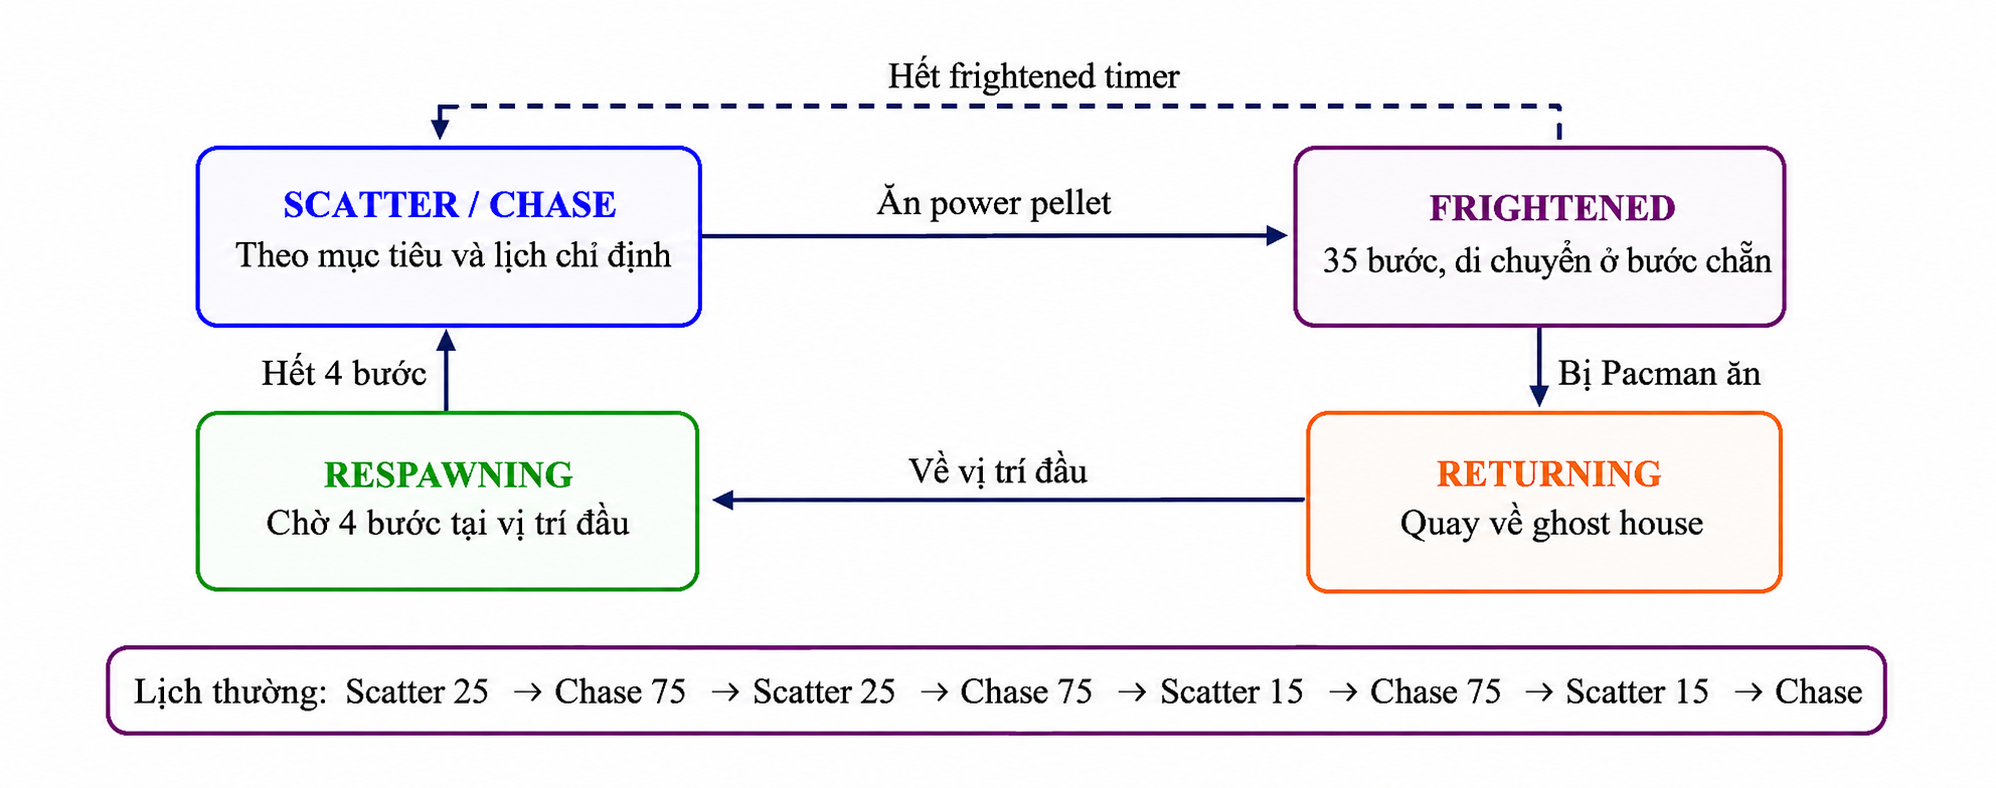
\includegraphics[width=0.94\textwidth]{image/hinh_3_3.png}
    \caption{Các trạng thái hoạt động và quá trình chuyển đổi của ma trong môi trường Mini Pacman.}
    \label{fig:ghost-state-flow}
\end{figure}

Episode kết thúc khi Pacman ăn hết 62 food, mất mạng cuối cùng hoặc đạt giới hạn 700 bước. Nếu Pacman bị bắt nhưng vẫn còn mạng, episode tiếp tục: Pacman và ba ma trở về vị trí xuất phát, còn food và bonus fruit đã ăn không được khôi phục. Do đó, tiến độ thu thập vật phẩm được giữ lại qua các lần mất mạng trong cùng một episode.

\subsection{Mô hình hóa bài toán học tăng cường}

Để lựa chọn action, tác tử cần nắm được vị trí của Pacman, vị trí và trạng thái của các ma, lượng food còn lại, số mạng và thời gian hiệu lực của power pellet. Môi trường mã hóa những thông tin này theo hai cách. Q-Learning sử dụng state dạng tuple, còn DQN và Double DQN nhận state dưới dạng vector số thực.

\subsubsection{Không gian và biểu diễn trạng thái}

State gốc gồm 17 giá trị, bao gồm hai tọa độ của Pacman, sáu tọa độ của ba ma, ba cờ returning, ba respawn timer, frightened timer, số mạng còn lại và một food mask. Q-Learning dùng trực tiếp tuple này làm khóa của Q-table. Mỗi khóa gắn với bốn Q-value tương ứng với bốn action. Các giá trị được khởi tạo bằng $0$ khi state xuất hiện lần đầu.

Đối với DQN và Double DQN, state được mở rộng thành vector 92 chiều. Food mask được tách thành 62 bit rồi ghép thêm thông tin về food gần nhất, ma đang hoạt động gần nhất, action hợp lệ và action nguy hiểm. Hai cách biểu diễn state được minh họa trong \figref{fig:state-representation}. Cấu trúc chi tiết của vector 92 chiều được trình bày trong \tabref{tab:state-vector}.

\begin{figure}[H]
    \centering
    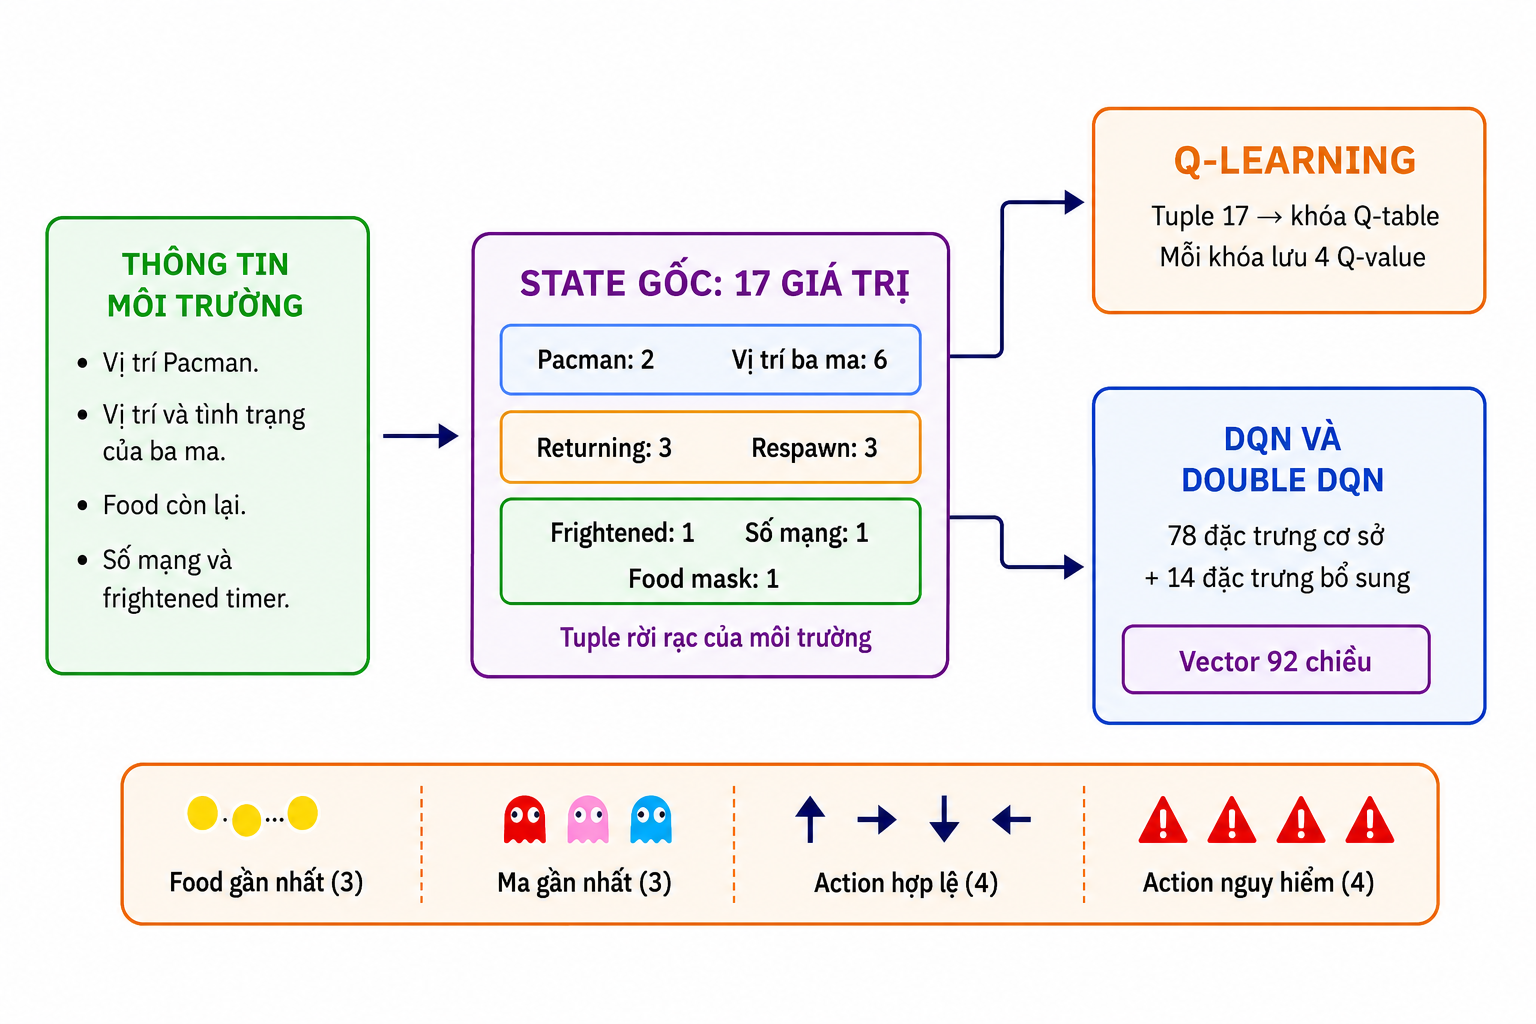
\includegraphics[width=0.94\textwidth]{image/hinh_3_4.png}
    \caption{Hai cách biểu diễn state được sử dụng cho Q-Learning và các phương pháp deep Q-learning.}
    \label{fig:state-representation}
\end{figure}

\begin{table}[H]
    \centering
    \renewcommand{\arraystretch}{1.16}
    \small
    \begin{tabularx}{0.96\textwidth}{@{}
        >{\raggedright\arraybackslash}p{3.7cm}
        >{\centering\arraybackslash}p{1.6cm}
        >{\raggedright\arraybackslash}X
    @{}}
        \toprule
        \textbf{Nhóm đặc trưng} & \textbf{Số chiều} & \textbf{Cách biểu diễn} \\
        \midrule
        Vị trí Pacman & 2 & Tọa độ hàng và cột, mỗi giá trị chia cho 14. \\
        Vị trí ba ma & 6 & Hai tọa độ cho mỗi ma, mỗi giá trị chia cho 14. \\
        Returning flags & 3 & Một cờ $0/1$ cho mỗi ma. \\
        Respawn timers & 3 & Một bộ đếm cho mỗi ma, chia cho 4. \\
        Số mạng còn lại & 1 & Số mạng chia cho 3. \\
        Frightened timer & 1 & Bộ đếm frightened chia cho 35. \\
        Food mask & 62 & Một cờ $0/1$ cho mỗi vị trí food cố định. \\
        Food gần nhất & 3 & Độ lệch hàng, độ lệch cột chia cho 14 và khoảng cách Manhattan chia cho 28. \\
        Ma đang hoạt động gần nhất & 3 & Độ lệch hàng, độ lệch cột chia cho 14 và khoảng cách Manhattan chia cho 28. \\
        Action hợp lệ & 4 & Bốn cờ $0/1$ theo thứ tự lên, phải, xuống và trái. \\
        Action nguy hiểm & 4 & Bốn cờ $0/1$, cho biết vị trí sau action có cách ma không quá hai ô Manhattan hay không. \\
        \midrule
        Tổng cộng & 92 & 78 đặc trưng cơ sở và 14 đặc trưng bổ sung. \\
        \bottomrule
    \end{tabularx}
    \caption{Cấu trúc vector state của DQN và Double DQN \cite{DRLPacmanGitHub}.}
    \label{tab:state-vector}
\end{table}

Food và ma gần nhất được lựa chọn theo maze distance, nhưng thành phần khoảng cách tương đối lưu trong vector là Manhattan distance. Khi xác định ma gần nhất, các ma đang returning hoặc respawning được loại bỏ. Nếu frightened timer lớn hơn $0$, bốn cờ action nguy hiểm đều bằng $0$. Power pellet không cần nhóm riêng vì bốn vị trí này cố định trong 62 food bit. Ảnh hưởng sau khi ăn được thể hiện qua frightened timer. Tường và ghost door cũng không được mã hóa thành toàn bộ bản đồ vì bố cục không thay đổi, trong khi bốn cờ action hợp lệ cung cấp thông tin di chuyển tại vị trí hiện tại \cite{DRLPacmanGitHub}.

Biểu diễn trên không chứa tình trạng của bonus fruit, số bước hiện tại, chế độ scatter/chase, action trước đó của Pacman và action trước đó của các ma. Các biến này vẫn tham gia vào luật chuyển trạng thái hoặc điều kiện kết thúc. Vì vậy, state được lựa chọn đáp ứng phạm vi thực nghiệm của đề tài nhưng không mô tả toàn bộ biến nội bộ của môi trường. Đầu vào của cả ba phương pháp được tạo từ dữ liệu trạng thái, không sử dụng ảnh chụp màn hình.

\subsubsection{Không gian hành động}

Không gian action gồm bốn hướng theo thứ tự lên, phải, xuống và trái. Tác tử không có action đứng yên. Cả Q-Learning, DQN và Double DQN đều có thể chọn một trong bốn action, kể cả khi hướng đó bị tường hoặc ghost door chặn. Trong trường hợp này, Pacman giữ nguyên vị trí và nhận penalty va tường. Bốn cờ action hợp lệ trong vector state chỉ cung cấp thông tin cho Q-network, không giới hạn trực tiếp action được chọn.

Trong training, action được chọn theo $\epsilon$-greedy. Ở exploration, tác tử chọn ngẫu nhiên một trong bốn action. Ở exploitation, action có Q-value lớn nhất được sử dụng. Trong evaluation, $\epsilon$ được đặt bằng $0$ để loại bỏ exploration.

\subsubsection{Thiết kế phần thưởng}

Reward vừa phản ánh kết quả của các sự kiện trong trò chơi, vừa định hướng Pacman thu thập food và duy trì khoảng cách an toàn với ma. Các thành phần có thể được cộng trong cùng một environment step. Chẳng hạn, khi Pacman ăn power pellet, reward của food và reward bổ sung của power pellet cùng được ghi nhận. Các giá trị chính xác được trình bày trong \tabref{tab:reward-design}.

\begin{table}[H]
    \centering
    % Compact this long table slightly so its caption stays clear of the footer.
    \renewcommand{\arraystretch}{1.05}
    \captionsetup{skip=5pt}
    \small
    \begin{tabularx}{0.92\textwidth}{@{}
        >{\raggedright\arraybackslash}X
        >{\centering\arraybackslash}p{2.6cm}
    @{}}
        \toprule
        \textbf{Thành phần reward} & \textbf{Giá trị cộng thêm} \\
        \midrule
        Mỗi environment step & $-0{,}10$ \\
        Va vào tường hoặc ghost door & $-1{,}00$ \\
        Ăn một food & $+10{,}00$ \\
        Food là power pellet & $+50{,}00$ \\
        Ăn một bonus fruit & $+100{,}00$ \\
        Ăn một ma đang frightened & $+200{,}00$ \\
        Ăn hết food và thắng episode & $+100{,}00$ \\
        Bị ma bắt và mất một mạng & $-50{,}00$ \\
        Không thắng và không bị ma bắt trong bước hiện tại & $+0{,}02$ \\
        Tiến gần food gần nhất khi chưa ăn vật phẩm & $+0{,}03$ \\
        Đi xa food gần nhất khi chưa ăn vật phẩm & $-0{,}03$ \\
        Tăng khoảng cách tới ma gần nhất & $+0{,}05$ \\
        Tiến gần ma trong vùng nguy hiểm không quá năm ô & $-0{,}10$ \\
        Chạm giới hạn 700 bước & $-10{,}00$ \\
        \bottomrule
    \end{tabularx}
    \caption{Các thành phần reward của môi trường Mini Pacman \cite{DRLPacmanGitHub}.}
    \label{tab:reward-design}
\end{table}

Reward tiến gần hoặc đi xa food chỉ được áp dụng khi Pacman không ăn food hay bonus fruit ở bước hiện tại và trên bản đồ vẫn còn food. Reward tồn tại được cộng sau khi kiểm tra điều kiện thắng và bị bắt, nhưng trước khi kiểm tra giới hạn 700 bước. Vì vậy, bước chạm giới hạn vẫn có thể nhận $+0{,}02$ trước khi nhận penalty timeout. Các thành phần reward dựa trên khoảng cách tới food và ma sử dụng maze distance. Riêng cờ action nguy hiểm trong vector state sử dụng Manhattan distance sau khi thử action.

\subsection{Cài đặt các thuật toán}

Cả ba phương pháp đều nhận cùng loại phản hồi từ môi trường nhưng khác nhau ở cơ chế học. Q-Learning cập nhật trực tiếp Q-table sau mỗi transition. DQN và Double DQN đưa transition vào replay buffer rồi lấy mẫu theo mini-batch để cập nhật Q-network \cite{DRLPacmanGitHub}.

\subsubsection{Q-Learning}

Nguyên lý lựa chọn action và cập nhật Q-table đã được trình bày tại Mục 2.2, đồng thời được minh họa trong \figref{fig:q-learning-principle}. Khi áp dụng vào Mini Pacman, tuple state gồm 17 giá trị được dùng làm khóa của Q-table. Mỗi khóa lưu bốn Q-value tương ứng với bốn action. Sau mỗi transition, Q-value của cặp state--action vừa thực hiện được cập nhật theo phương trình~\eqref{eq:q-learning-update}. Nếu transition kết thúc episode, thành phần bootstrap bằng $0$. Ngược lại, target sử dụng Q-value lớn nhất của state kế tiếp.

Q-Learning lựa chọn action theo chiến lược $\epsilon$-greedy và giảm epsilon sau mỗi episode. Tại từng mốc checkpoint, hệ thống lưu Q-table, epsilon, trạng thái của bộ sinh số ngẫu nhiên và tiến độ huấn luyện. Nhờ đó, thí nghiệm có thể tiếp tục từ mốc gần nhất nếu bị gián đoạn. Mô hình cuối chỉ chứa Q-table đã học để phục vụ evaluation và demo.

\subsubsection{DQN}

DQN sử dụng mạng multilayer perceptron với đầu vào là vector state 92 chiều và đầu ra là bốn Q-value. Mạng có hai hidden layer, mỗi layer gồm 128 neuron và sử dụng hàm kích hoạt ReLU. Output layer không dùng hàm kích hoạt. Online network và target network có cùng kiến trúc, mỗi mạng gồm 28.932 tham số. Cấu trúc mạng và mối quan hệ giữa hai nhánh được minh họa trong \figref{fig:q-network-architecture}.

\begin{figure}[H]
    \centering
    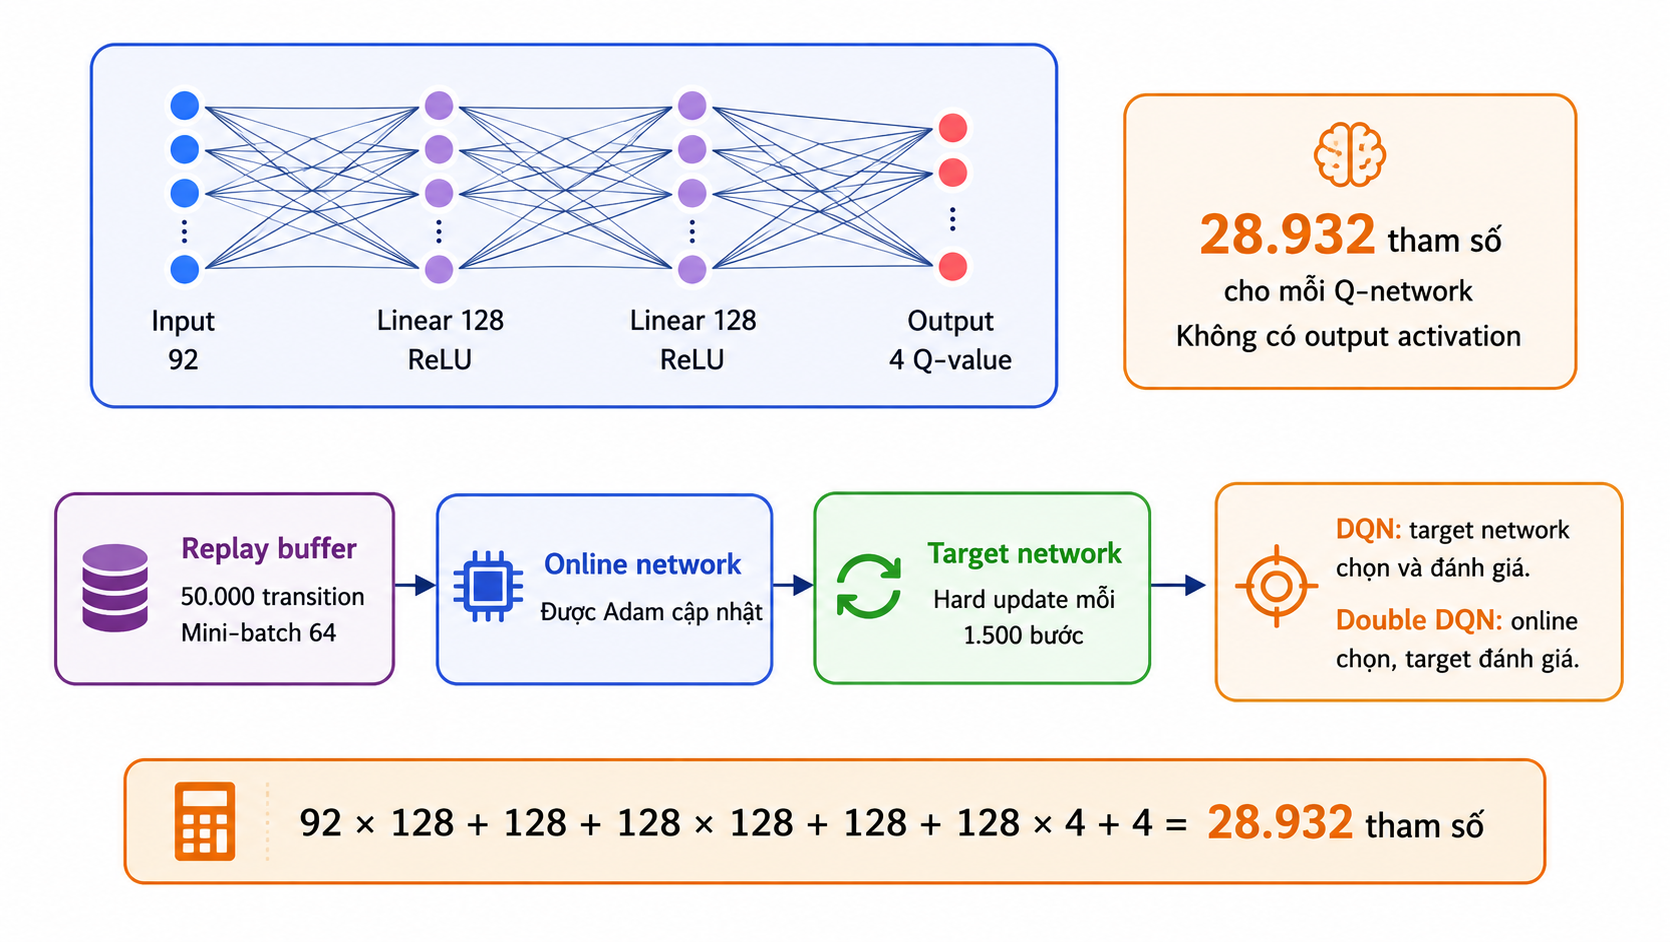
\includegraphics[width=0.94\textwidth]{image/hinh_3_5.png}
    \caption{Kiến trúc Q-network và vai trò của online network, target network trong hai phương pháp.}
    \label{fig:q-network-architecture}
\end{figure}

Mỗi transition gồm state vector, action, reward, next-state vector và cờ kết thúc. Các transition được lưu trong replay buffer hoạt động theo cơ chế FIFO với sức chứa 50.000 mẫu. Việc học bắt đầu sau khi tác tử tích lũy đủ 10.000 environment step. Ở mỗi lần cập nhật, hệ thống lấy ngẫu nhiên 64 transition không lặp trong cùng mini-batch để tối ưu online network. Sau mỗi 1.500 environment step, toàn bộ trọng số của online network được sao chép sang target network.

Online network được tối ưu bằng Adam với learning rate tương ứng của từng cấu hình. Hàm \texttt{SmoothL1Loss} được áp dụng cho TD error, còn gradient norm được giới hạn ở $10{,}0$. DQN target được tính theo phương trình~\eqref{eq:dqn-target}. Epsilon chỉ giảm sau khi online network thực hiện một lần cập nhật thành công. Vì vậy, epsilon được giữ nguyên trong 10.000 bước thu thập dữ liệu ban đầu.

Mô hình cuối chỉ lưu state dictionary của online network. Khi mô hình được tải để evaluation hoặc demo, target network được đồng bộ lại từ online network. Trong khi đó, checkpoint phục vụ việc tiếp tục training nên lưu thêm target network, optimizer, replay buffer, epsilon, trạng thái bộ sinh số ngẫu nhiên và tiến độ huấn luyện.

\subsubsection{Double DQN}

Double DQN giữ nguyên vector đầu vào, kiến trúc mạng, optimizer, loss, replay buffer, chiến lược exploration và lịch cập nhật target network của DQN. Điểm khác biệt duy nhất là cách tính target cho next state. Online network chọn action theo phương trình~\eqref{eq:ddqn-action-selection}. Sau đó, target network đánh giá action đã chọn theo phương trình~\eqref{eq:ddqn-target}. TD error vẫn được tối ưu bằng \texttt{SmoothL1Loss}, nhưng DQN target được thay bằng Double DQN target. Các siêu tham số còn lại được giữ giống DQN tại cùng learning rate.

\subsection{Thiết kế thực nghiệm}

Thực nghiệm gồm chín cấu hình, được tạo từ ba thuật toán và ba giá trị learning rate. Trong phạm vi từng thuật toán, chỉ learning rate được thay đổi. Bản đồ, số episode, seed, lịch evaluation và những thiết lập còn lại được giữ cố định. Cách bố trí này giúp đánh giá ảnh hưởng của learning rate mà không làm thay đổi đồng thời các yếu tố khác.

\subsubsection{Cấu hình và siêu tham số}

Ba giá trị learning rate được khảo sát là $0{,}0001$, $0{,}0005$ và $0{,}001$. Trong Q-Learning, tham số này điều khiển trực tiếp mức cập nhật của Q-table. Với DQN và Double DQN, learning rate thuộc optimizer Adam. Do hai cơ chế học khác nhau, kết quả chỉ được so sánh giữa các learning rate trong cùng một thuật toán. Một giá trị giống nhau không có nghĩa là Q-table và Q-network thay đổi với mức độ tương đương.

\begin{itemize}
    \item \textbf{Thiết bị huấn luyện:} laptop cá nhân MSI Cyborg 15, trang bị GPU NVIDIA GeForce RTX 4050 Laptop GPU với 6 GB VRAM.
\end{itemize}

Các tham số chung của chín thí nghiệm được trình bày trong \tabref{tab:common-hyperparameters}.

\begin{table}[H]
    \centering
    \renewcommand{\arraystretch}{1.18}
    \small
    \begin{tabularx}{0.88\textwidth}{@{}
        >{\raggedright\arraybackslash}X
        >{\centering\arraybackslash}p{4.4cm}
    @{}}
        \toprule
        \textbf{Tham số} & \textbf{Giá trị} \\
        \midrule
        Learning rate & $0{,}0001$, $0{,}0005$ và $0{,}001$ \\
        Số episode training & 20.000 \\
        Discount factor & $0{,}99$ \\
        Layout & \texttt{medium}, $15\times15$ ô \\
        Số bước tối đa mỗi episode & 700 \\
        Số mạng sống & 3 \\
        Số ma & 3 \\
        Training seed & 42 \\
        Checkpoint interval & 1.000 episode \\
        Evaluation interval & 1.000 episode \\
        Số episode mỗi lần evaluation & 20 \\
        Evaluation seed & 10042 \\
        \bottomrule
    \end{tabularx}
    \caption{Các tham số chung của chín cấu hình thực nghiệm \cite{DRLPacmanGitHub}.}
    \label{tab:common-hyperparameters}
\end{table}

Các thiết lập riêng của từng phương pháp được tổng hợp trong \tabref{tab:algorithm-hyperparameters}. DQN và Double DQN dùng cùng cấu hình. Sự khác biệt giữa chúng nằm ở cách tính target.

\begin{table}[H]
    \centering
    \renewcommand{\arraystretch}{1.15}
    \footnotesize
    \begin{tabularx}{\textwidth}{@{}
        >{\raggedright\arraybackslash}p{3.5cm}
        >{\centering\arraybackslash}p{3.2cm}
        >{\centering\arraybackslash}X
        >{\centering\arraybackslash}X
    @{}}
        \toprule
        \textbf{Tham số} & \textbf{Q-Learning} & \textbf{DQN} & \textbf{Double DQN} \\
        \midrule
        Epsilon ban đầu & $1{,}0$ & $1{,}0$ & $1{,}0$ \\
        Epsilon nhỏ nhất & $0{,}05$ & $0{,}02$ & $0{,}02$ \\
        Epsilon decay & $0{,}99985$/episode & $0{,}999997$/update & $0{,}999997$/update \\
        Kích thước hidden layer & Không sử dụng & 128, 128 & 128, 128 \\
        Batch size & Không sử dụng & 64 & 64 \\
        Replay capacity & Không sử dụng & 50.000 & 50.000 \\
        Learning starts & Không sử dụng & 10.000 bước & 10.000 bước \\
        Target update interval & Không sử dụng & 1.500 bước & 1.500 bước \\
        Optimizer & Không sử dụng & Adam & Adam \\
        Loss & Không sử dụng & SmoothL1 & SmoothL1 \\
        Gradient clipping & Không sử dụng & Max norm $10{,}0$ & Max norm $10{,}0$ \\
        \bottomrule
    \end{tabularx}
    \caption{Các tham số riêng của Q-Learning, DQN và Double DQN \cite{DRLPacmanGitHub}.}
    \label{tab:algorithm-hyperparameters}
\end{table}

Training seed, evaluation seed và cấu hình của từng thí nghiệm được giữ cố định để hỗ trợ tái lập kết quả.

\subsubsection{Quy trình huấn luyện và đánh giá}

Mỗi thí nghiệm bắt đầu bằng việc khởi tạo môi trường và tác tử theo cấu hình tương ứng. Trong từng episode, tác tử liên tục tương tác với môi trường để cập nhật Q-table hoặc Q-network. Các metric training được ghi lại sau mỗi episode. Cứ 1.000 episode, hệ thống lưu checkpoint và thực hiện một lần evaluation độc lập. Quy trình đầy đủ được tóm tắt trong \figref{fig:experiment-process}.

\begin{figure}[H]
    \centering
    \resizebox{0.94\textwidth}{!}{%
    \begin{tikzpicture}[x=1cm,y=1cm,font=\fontsize{8.5}{10.2}\selectfont]
            \node[chthreeorange, minimum width=10.5cm, minimum height=0.75cm] at (7.6,4.35)
                {9 thí nghiệm $=$ 3 thuật toán $\times$ 3 learning rate: $0{,}0001$, $0{,}0005$, $0{,}001$};
    
            \foreach \x/\n/\col in {1.25/1/orange,4.35/2/blue,7.45/3/violet,10.55/4/green,13.65/5/orange}{
                \fill[\col!72] (\x,3.25) circle (0.30);
                \node[font=\bfseries,text=white] at (\x,3.25) {\n};
            }
            \draw[chthreeflow] (1.58,3.25) -- (4.02,3.25);
            \draw[chthreeflow] (4.68,3.25) -- (7.12,3.25);
            \draw[chthreeflow] (7.78,3.25) -- (10.22,3.25);
            \draw[chthreeflow] (10.88,3.25) -- (13.32,3.25);
    
            \node[chthreeorange, minimum width=2.6cm, minimum height=1.65cm] at (1.25,1.8)
                {\textbf{Khởi tạo}\\Layout medium\\Training seed 42};
            \node[chthreeblue, minimum width=2.6cm, minimum height=1.65cm] at (4.35,1.8)
                {\textbf{Training}\\20.000 episode\\$\epsilon$-greedy};
            \node[chthreepurple, minimum width=2.6cm, minimum height=1.65cm] at (7.45,1.8)
                {\textbf{Mỗi 1.000 episode}\\Lưu checkpoint\\Chạy evaluation};
            \node[chthreegreen, minimum width=2.6cm, minimum height=1.65cm] at (10.55,1.8)
                {\textbf{Evaluation}\\20 episode\\$\epsilon=0$, seed 10042};
            \node[chthreeorange, minimum width=2.6cm, minimum height=1.65cm] at (13.65,1.8)
                {\textbf{Hoàn tất}\\Lưu model cuối\\Ghi nhận metric};
    
            \node[chthreepurple, minimum width=10.2cm, minimum height=0.65cm] at (7.6,0.35)
                {Evaluation không cập nhật Q-table, replay buffer, optimizer hoặc tham số network.};
        \end{tikzpicture}
    }
    \caption{Quy trình training, lưu checkpoint, evaluation và lưu mô hình cuối.}
    \label{fig:experiment-process}
\end{figure}

Trong mỗi lần evaluation, $\epsilon$ được đặt bằng $0$ và tác tử chạy 20 episode với evaluation seed 10042. Tác tử chỉ sử dụng cơ chế chọn action của policy hiện tại. Q-table, replay buffer, optimizer và tham số mạng đều không được cập nhật. Sau 20.000 episode training, hệ thống lưu mô hình cuối cùng và ghi nhận kết quả của lần evaluation cuối.

Checkpoint và final model phục vụ hai mục đích khác nhau. Checkpoint lưu các thành phần cần thiết để tiếp tục training từ mốc gần nhất. Final model chỉ giữ Q-table đối với Q-Learning hoặc trọng số online network đối với DQN và Double DQN, phù hợp cho evaluation và demo.

\subsubsection{Tiêu chí đánh giá}

Mỗi lần evaluation gồm 20 episode với $\epsilon=0$. Thiết lập này giúp kết quả phản ánh trực tiếp policy đã học mà không bị ảnh hưởng bởi hành động thăm dò. Gọi $N=20$ là số episode trong một lần evaluation. Ở episode thứ $i$, $R_i$, $T_i$ và $F_i$ lần lượt biểu thị reward tích lũy, số bước thực hiện và số food đã ăn. Các tiêu chí đánh giá được xây dựng từ ba đại lượng này.

\noindent\textbf{Reward trung bình.}
\begin{equation}
    \overline{R}=\frac{1}{N}\sum_{i=1}^{N}R_i.
    \label{eq:average-reward}
\end{equation}
Đại lượng $\overline{R}$ phản ánh reward tích lũy trung bình của tác tử. Do reward có thể được cộng từ nhiều sự kiện trong cùng một bước, chỉ số này cần được đọc cùng win rate, completion rate và số bước trung bình thay vì dùng riêng để kết luận về chất lượng policy.

\noindent\textbf{Số bước trung bình.}
\begin{equation}
    \overline{T}=\frac{1}{N}\sum_{i=1}^{N}T_i.
    \label{eq:average-steps}
\end{equation}
$\overline{T}$ cho biết độ dài trung bình của một episode trước khi tác tử chiến thắng, mất mạng cuối cùng hoặc đạt giới hạn bước. Số bước lớn không đồng nghĩa với policy tốt hơn nên chỉ số này phải được xem cùng win rate và completion rate.

\noindent\textbf{Số food ăn được trung bình.}
\begin{equation}
    \overline{F}=\frac{1}{N}\sum_{i=1}^{N}F_i.
    \label{eq:average-food}
\end{equation}
$\overline{F}$ biểu thị lượng food trung bình tác tử thu thập được trong một episode, qua đó cho thấy mức tiến triển của tác tử trên bản đồ.

\noindent\textbf{Completion rate trung bình.}
\begin{equation}
    \overline{C}=\frac{1}{N}\sum_{i=1}^{N}\left(\frac{F_i}{62}\times100\%\right).
    \label{eq:average-completion}
\end{equation}
Mỗi episode có tổng cộng 62 food. Vì vậy, $F_i/62$ là tỷ lệ bản đồ được hoàn thành trong episode thứ $i$, còn $\overline{C}$ là tỷ lệ hoàn thành trung bình của toàn bộ 20 episode.

\noindent\textbf{Win rate.}
\begin{equation}
    \mathrm{WinRate}=\frac{1}{N}\sum_{i=1}^{N}\mathbf{1}(F_i=62)\times100\%.
    \label{eq:evaluation-win-rate}
\end{equation}
Hàm chỉ thị $\mathbf{1}(F_i=62)$ nhận giá trị $1$ khi tác tử ăn hết 62 food và chiến thắng, ngược lại nhận giá trị $0$. Win rate trong evaluation được tính độc lập trên 20 episode tại từng mốc. Chỉ số này khác với win rate tích lũy trong lịch sử training.

\noindent\textbf{Reward tốt nhất.}
\begin{equation}
    R_{\max}=\max_{1\leq i\leq N}R_i.
    \label{eq:best-reward}
\end{equation}
$R_{\max}$ ghi nhận reward tích lũy lớn nhất trong 20 episode, thể hiện kết quả tốt nhất mà policy đạt được ở lần evaluation đó.

\noindent\textbf{Completion rate tốt nhất.}
\begin{equation}
    C_{\max}=\max_{1\leq i\leq N}\left(\frac{F_i}{62}\times100\%\right).
    \label{eq:best-completion}
\end{equation}
$C_{\max}$ là tỷ lệ hoàn thành lớn nhất trong 20 episode, cho biết policy đã tiến gần đến việc hoàn thành bản đồ nhất ở mức nào.

Đối với DQN và Double DQN, loss được tính bằng \texttt{SmoothL1Loss} theo phương trình~\eqref{eq:dqn-loss}. Q-Learning không sử dụng chỉ số này vì không huấn luyện mạng nơ-ron. Hệ thống còn thống kê số episode kết thúc do chiến thắng, mất mạng cuối cùng hoặc đạt giới hạn bước. \tabref{tab:evaluation-metrics} tóm tắt toàn bộ tiêu chí được sử dụng.

\begin{table}[H]
    \centering
    \renewcommand{\arraystretch}{1.08}
    \captionsetup{skip=5pt}
    \small
    \begin{tabularx}{0.96\textwidth}{@{}
        >{\raggedright\arraybackslash}p{3.4cm}
        >{\raggedright\arraybackslash}X
    @{}}
        \toprule
        \textbf{Metric} & \textbf{Ý nghĩa và cách tính} \\
        \midrule
        Average reward & Reward tích lũy trung bình của 20 episode evaluation, được đọc cùng win rate, completion rate và số bước. \\
        Average steps & Số bước trung bình trước khi episode kết thúc, được đọc cùng win rate và completion rate. \\
        Average food eaten & Số food được ăn trung bình trong 20 episode. \\
        Average completion rate & Trung bình tỷ lệ food đã ăn trên tổng số 62 food của từng episode. \\
        Win rate & Số episode chiến thắng chia cho 20 episode evaluation. \\
        Loss & Trung bình \texttt{SmoothL1Loss} của các update trong một episode training, chỉ có ở DQN và Double DQN. \\
        Best reward & Reward lớn nhất trong 20 episode evaluation. \\
        Best completion rate & Completion rate lớn nhất trong 20 episode evaluation. \\
        Wins, caught, timeout & Số episode kết thúc do thắng, mất mạng cuối cùng hoặc đạt giới hạn bước. \\
        \bottomrule
    \end{tabularx}
    \caption{Các tiêu chí được sử dụng để đánh giá kết quả thực nghiệm.}
    \label{tab:evaluation-metrics}
\end{table}

Lần đánh giá cuối sử dụng $\epsilon=0$ nên phản ánh policy đã học mà không trộn lẫn exploration.

\clearpage
\section{KẾT QUẢ THỰC NGHIỆM VÀ THẢO LUẬN}

\subsection{Kết quả đánh giá cuối}

Sau 20.000 episode training, cả chín cấu hình được evaluation độc lập trên 20 episode với $\epsilon=0$. Tất cả cấu hình sử dụng training seed 42 và evaluation seed 10042. Hai seed được tách riêng, còn evaluation seed được giữ cố định nhằm tăng tính nhất quán và khả năng tái lập kết quả. \tabref{tab:final-eval-results} tổng hợp kết quả của lần evaluation cuối tại episode 20.000 \cite{DRLPacmanGitHub}.

\begin{table}[H]
    \centering
    \renewcommand{\arraystretch}{1.2}
    \small
    \begin{tabularx}{\textwidth}{@{}
        >{\raggedright\arraybackslash}p{2.4cm}
        >{\centering\arraybackslash}p{1.1cm}
        >{\centering\arraybackslash}p{1.9cm}
        >{\centering\arraybackslash}p{2.6cm}
        >{\centering\arraybackslash}p{1.4cm}
        >{\centering\arraybackslash}p{1.5cm}
        >{\centering\arraybackslash}X
    @{}}
        \toprule
        \textbf{Thuật toán} & \textbf{LR} & \textbf{Reward Avg} & \textbf{Completion Avg} & \textbf{Win Rate} & \textbf{Steps Avg} & \textbf{Completion Max} \\
        \midrule
        Double DQN & $0{,}0001$ & $1247{,}154$ & $99{,}76\%$ & $95\%$ & $148{,}30$ & $100\%$ \\
        Double DQN & $0{,}0005$ & $1312{,}231$ & $99{,}27\%$ & $85\%$ & $153{,}60$ & $100\%$ \\
        Double DQN & $0{,}001$ & $1553{,}422$ & $99{,}27\%$ & $65\%$ & $211{,}65$ & $100\%$ \\
        DQN & $0{,}0001$ & $1125{,}694$ & $98{,}55\%$ & $75\%$ & $157{,}85$ & $100\%$ \\
        DQN & $0{,}0005$ & $1254{,}443$ & $99{,}84\%$ & $95\%$ & $138{,}90$ & $100\%$ \\
        DQN & $0{,}001$ & $1148{,}294$ & $98{,}71\%$ & $75\%$ & $161{,}85$ & $100\%$ \\
        Q-Learning & $0{,}0001$ & $61{,}960$ & $26{,}29\%$ & $0\%$ & $99{,}25$ & $51{,}61\%$ \\
        Q-Learning & $0{,}0005$ & $134{,}079$ & $42{,}66\%$ & $0\%$ & $124{,}05$ & $51{,}61\%$ \\
        Q-Learning & $0{,}001$ & $165{,}472$ & $46{,}29\%$ & $0\%$ & $134{,}40$ & $54{,}84\%$ \\
        \bottomrule
    \end{tabularx}
    \caption{Kết quả đánh giá hiệu năng cuối cùng của các thuật toán tại episode 20.000 \cite{DRLPacmanGitHub}.}
    \label{tab:final-eval-results}
\end{table}

Kết quả trong \tabref{tab:final-eval-results} cho thấy ba điểm chính:
\begin{itemize}
    \item \textbf{Khác biệt giữa phương pháp dạng bảng và phương pháp dùng mạng nơ-ron:} Q-Learning không thắng episode nào ở cả ba learning rate, trong khi DQN và Double DQN đạt win rate từ $65\%$ đến $95\%$. Trong thiết kế thực nghiệm hiện tại, các cấu hình sử dụng Q-network với state 92 chiều đạt kết quả cao hơn Q-Learning sử dụng Q-table với tuple state 17 giá trị. Do đầu vào khác nhau, chênh lệch này chưa thể được quy hoàn toàn cho thuật toán.
    \item \textbf{Hai cấu hình có win rate cao nhất:} DQN với $\mathrm{LR}=0{,}0005$ và Double DQN với $\mathrm{LR}=0{,}0001$ cùng đạt win rate $95\%$. DQN hoàn thành các episode evaluation với số bước trung bình thấp hơn, lần lượt là $138{,}90$ và $148{,}30$. Khi win rate và completion rate của hai cấu hình gần tương đương, chênh lệch này cho thấy DQN sử dụng ít bước hơn trong lần evaluation cuối. Dữ liệu hiện tại chưa đủ để khẳng định đây là đường đi ngắn nhất.
    \item \textbf{Quan hệ giữa reward và khả năng hoàn thành:} Double DQN với $\mathrm{LR}=0{,}001$ đạt reward trung bình cao nhất là $1553{,}422$ nhưng win rate chỉ đạt $65\%$. Kết quả cho thấy reward tích lũy cao không đồng nghĩa với khả năng hoàn thành màn chơi ổn định. Do log evaluation không tách reward theo từng loại sự kiện, chưa thể xác định chính xác thành phần tạo ra mức chênh lệch này.
\end{itemize}

\subsection{Phân tích quá trình huấn luyện}

Các đồ thị trong mục này sử dụng metric ghi nhận sau từng episode training và được làm mượt bằng trung bình trượt 50 episode để thể hiện xu hướng. Các bảng tại mốc 1.000, 5.000, 10.000, 15.000 và 20.000 episode sử dụng kết quả evaluation độc lập trên 20 episode với $\epsilon=0$ và seed 10042. Hai nguồn dữ liệu được trình bày song song nhằm phản ánh cả diễn biến trong quá trình training và hiệu năng của policy tại từng checkpoint. Các bảng tập trung vào ba cấu hình có kết quả cuối tốt nhất của từng thuật toán: Double DQN với $\mathrm{LR}=0{,}0001$, DQN với $\mathrm{LR}=0{,}0005$ và Q-Learning với $\mathrm{LR}=0{,}001$.

\subsubsection{Reward}

\begin{figure}[H]
    \centering
    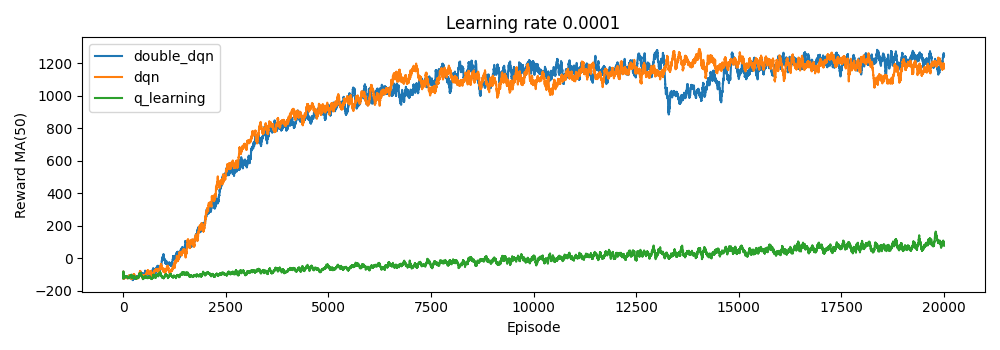
\includegraphics[width=0.85\textwidth]{image/reward_0001.png}
    \par\vspace{0.3cm}
    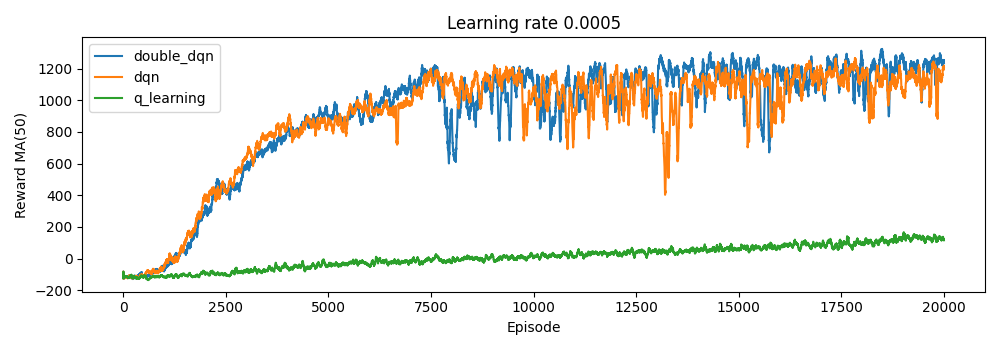
\includegraphics[width=0.85\textwidth]{image/reward_0005.png}
    \par\vspace{0.3cm}
    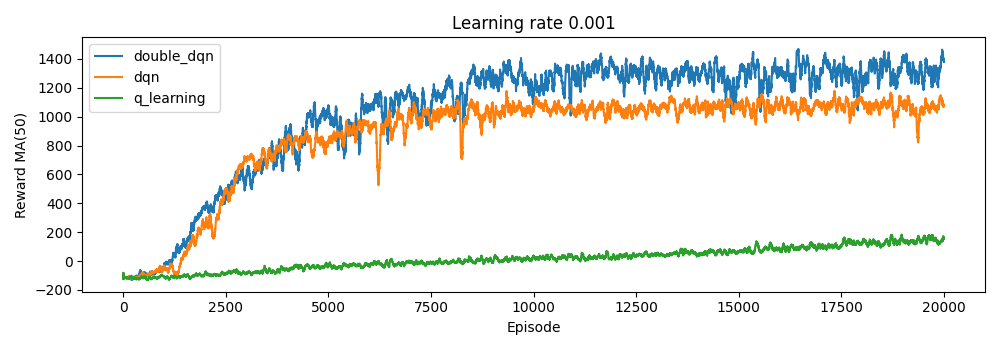
\includegraphics[width=0.85\textwidth]{image/reward_001.png}
    \caption{Reward trong quá trình training, được làm mượt bằng trung bình trượt 50 episode, với các mức learning rate lần lượt từ trên xuống dưới là $0{,}0001$, $0{,}0005$ và $0{,}001$.}
    \label{fig:reward-comparison}
\end{figure}

Reward tích lũy phản ánh tổng tác động của các sự kiện xảy ra trong một episode. Do nhiều thành phần reward có thể được cộng trong cùng một bước, chỉ số này cần được đọc cùng completion rate và win rate. \tabref{tab:reward-progress} trình bày reward trung bình từ các lần evaluation tại năm mốc training.

\begin{table}[H]
    \centering
    \renewcommand{\arraystretch}{1.2}
    \small
    \begin{tabular}{cccccc}
        \toprule
        \textbf{Cấu hình} & \makecell{\textbf{1.000}\\\textbf{episode}} & \makecell{\textbf{5.000}\\\textbf{episode}} & \makecell{\textbf{10.000}\\\textbf{episode}} & \makecell{\textbf{15.000}\\\textbf{episode}} & \makecell{\textbf{20.000}\\\textbf{episode}} \\
        \midrule
        Double DQN ($\mathrm{LR}=0{,}0001$) & $239{,}490$ & $946{,}191$ & $1195{,}874$ & $1159{,}812$ & $1247{,}154$ \\
        DQN ($\mathrm{LR}=0{,}0005$) & $302{,}023$ & $969{,}347$ & $982{,}988$ & $1257{,}292$ & $1254{,}443$ \\
        Q-Learning ($\mathrm{LR}=0{,}001$) & $-155{,}458$ & $-34{,}216$ & $16{,}860$ & $106{,}130$ & $165{,}472$ \\
        \bottomrule
    \end{tabular}
    \caption{Reward trung bình tại các mốc đánh giá.}
    \label{tab:reward-progress}
\end{table}

\figref{fig:reward-comparison} cho thấy reward training của DQN và Double DQN tăng nhanh trong giai đoạn đầu, sau đó dao động quanh mức cao. Tuy nhiên, reward tăng chưa đồng nghĩa với policy đã biết kết thúc màn chơi. Tại episode 5.000, Double DQN và DQN đạt reward evaluation lần lượt là $946{,}191$ và $969{,}347$, đồng thời đều thu thập hơn $95\%$ food. Dù vậy, hai cấu hình chỉ thắng lần lượt 1 và 0 trong 20 episode. Kết quả này cho thấy reward ở giai đoạn đó chủ yếu phản ánh khả năng thu thập phần lớn food và duy trì episode, còn khả năng hoàn thành vẫn chưa ổn định.

Đến episode 15.000, DQN đạt reward $1257{,}292$, completion rate $100\%$, win rate $100\%$ và chỉ cần trung bình $134{,}25$ bước. Sự thay đổi đồng thời của bốn chỉ số cho thấy policy không chỉ tạo reward cao hơn mà còn chuyển từ việc gần hoàn thành sang hoàn thành ổn định với ít bước hơn. Q-Learning cũng cải thiện reward từ $-155{,}458$ lên $165{,}472$, đi kèm completion rate tăng từ $8{,}39\%$ lên $46{,}29\%$. Tuy nhiên, win rate vẫn bằng $0\%$, nên mức reward tăng của Q-Learning chỉ phản ánh tiến bộ từng phần chứ chưa hình thành policy giải quyết hoàn chỉnh bài toán.

\subsubsection{Completion rate}

\begin{figure}[H]
    \centering
    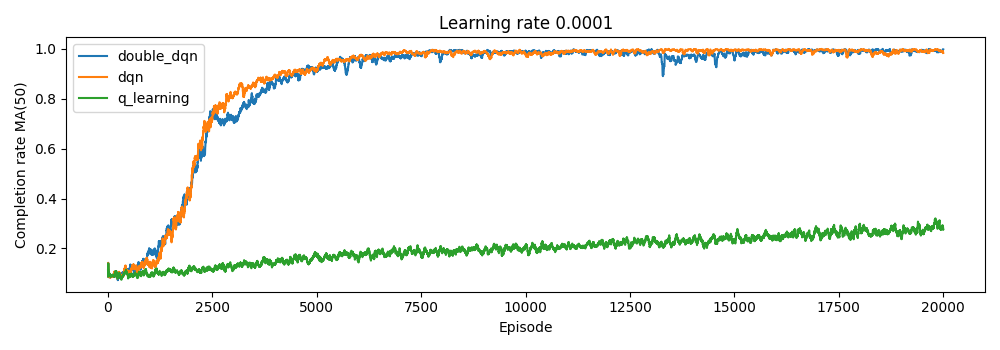
\includegraphics[width=0.85\textwidth]{image/completion_0001.png}
    \par\vspace{0.3cm}
    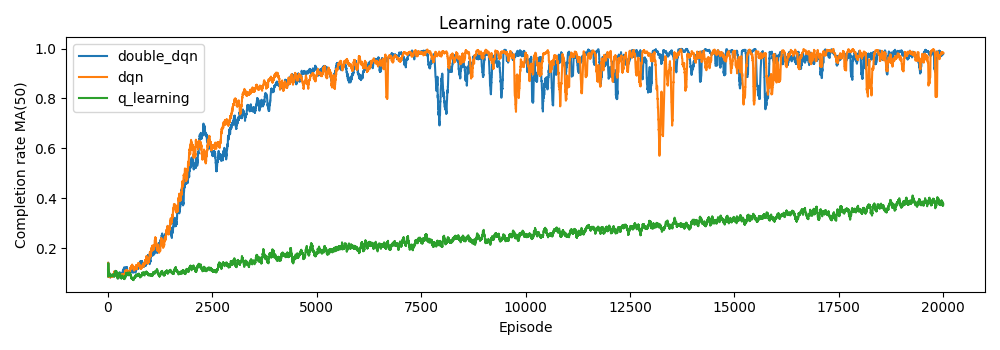
\includegraphics[width=0.85\textwidth]{image/completion_0005.png}
    \par\vspace{0.3cm}
    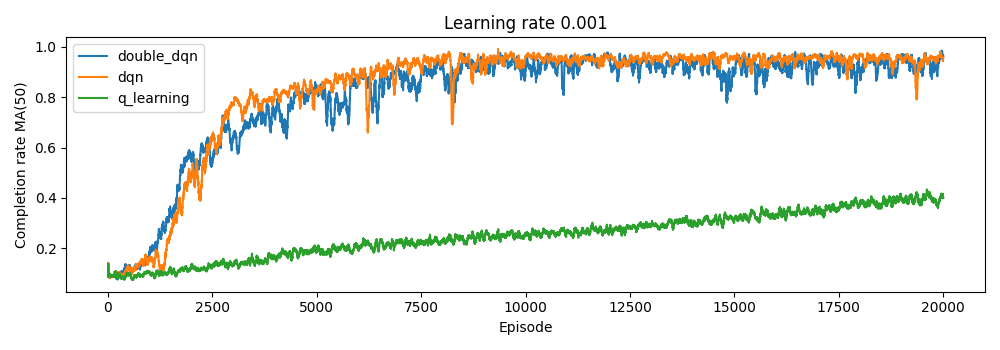
\includegraphics[width=0.85\textwidth]{image/completion_001.png}
    \caption{Completion rate trong quá trình training, được làm mượt bằng trung bình trượt 50 episode, với các mức learning rate lần lượt từ trên xuống dưới là $0{,}0001$, $0{,}0005$ và $0{,}001$.}
    \label{fig:completion-comparison}
\end{figure}

Completion rate biểu thị tỷ lệ food tác tử thu thập được trên tổng số 62 food của bản đồ. \tabref{tab:completion-progress} trình bày completion rate trung bình từ các lần evaluation tại năm mốc training.

\begin{table}[H]
    \centering
    \renewcommand{\arraystretch}{1.2}
    \small
    \begin{tabular}{cccccc}
        \toprule
        \textbf{Cấu hình} & \makecell{\textbf{1.000}\\\textbf{episode}} & \makecell{\textbf{5.000}\\\textbf{episode}} & \makecell{\textbf{10.000}\\\textbf{episode}} & \makecell{\textbf{15.000}\\\textbf{episode}} & \makecell{\textbf{20.000}\\\textbf{episode}} \\
        \midrule
        Double DQN ($\mathrm{LR}=0{,}0001$) & $49{,}11\%$ & $95{,}32\%$ & $99{,}03\%$ & $98{,}79\%$ & $99{,}76\%$ \\
        DQN ($\mathrm{LR}=0{,}0005$) & $58{,}71\%$ & $95{,}56\%$ & $91{,}21\%$ & $100{,}00\%$ & $99{,}84\%$ \\
        Q-Learning ($\mathrm{LR}=0{,}001$) & $8{,}39\%$ & $21{,}53\%$ & $27{,}74\%$ & $36{,}61\%$ & $46{,}29\%$ \\
        \bottomrule
    \end{tabular}
    \caption{Completion rate trung bình tại các mốc đánh giá.}
    \label{tab:completion-progress}
\end{table}

Completion rate giúp phân biệt hai mức độ học khác nhau: tìm được phần lớn food và thực sự hoàn thành episode. Tại episode 5.000, Double DQN đạt completion rate $95{,}32\%$ nhưng chỉ thắng 1/20 episode, còn DQN đạt $95{,}56\%$ nhưng không thắng episode nào. Như vậy, cả hai policy đã học được cách đi sâu vào mê cung và thu thập gần hết food, nhưng vẫn thường bị bắt trước khi lấy các food cuối cùng.

Khoảng cách giữa completion rate và win rate thu hẹp rõ rệt ở các checkpoint sau. DQN đạt đồng thời completion rate và win rate $100\%$ tại episode 15.000. Double DQN kết thúc training với completion rate $99{,}76\%$ và 19/20 episode chiến thắng. Ngược lại, Q-Learning tăng đều từ $8{,}39\%$ lên $46{,}29\%$ nhưng cả 20 episode evaluation cuối đều kết thúc do bị bắt. Q-Learning vì thế có học được hành vi thu thập food tốt hơn theo thời gian, song mức cải thiện chưa đủ để hoàn thành bản đồ.

\subsubsection{Win rate}

\begin{figure}[H]
    \centering
    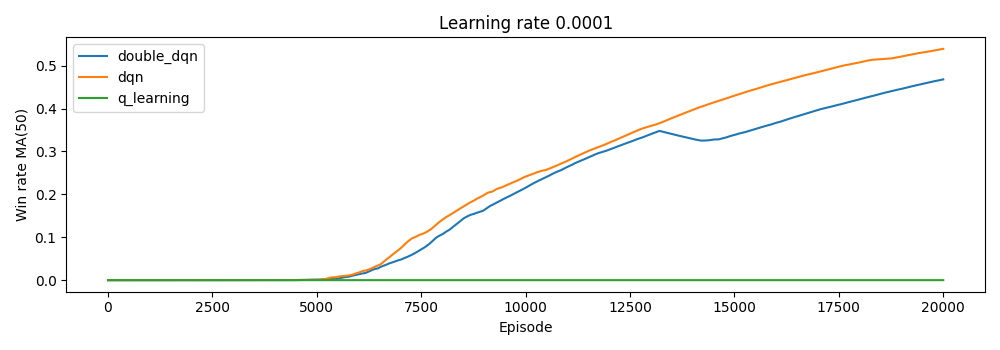
\includegraphics[width=0.85\textwidth]{image/win_rate_0001.png}
    \par\vspace{0.3cm}
    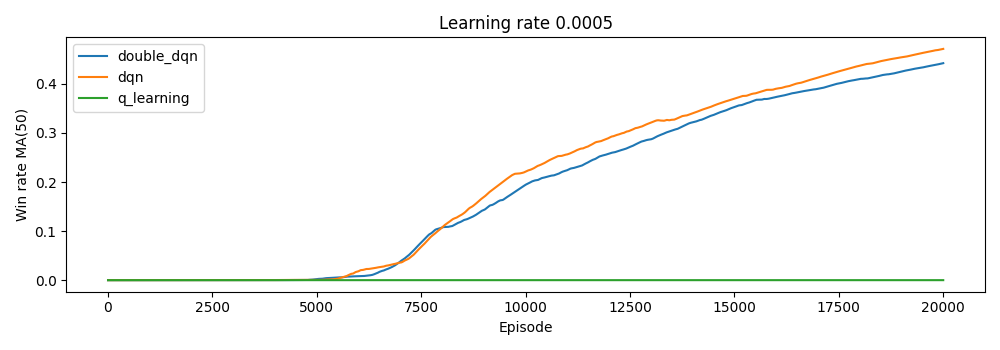
\includegraphics[width=0.85\textwidth]{image/win_rate_0005.png}
    \par\vspace{0.3cm}
    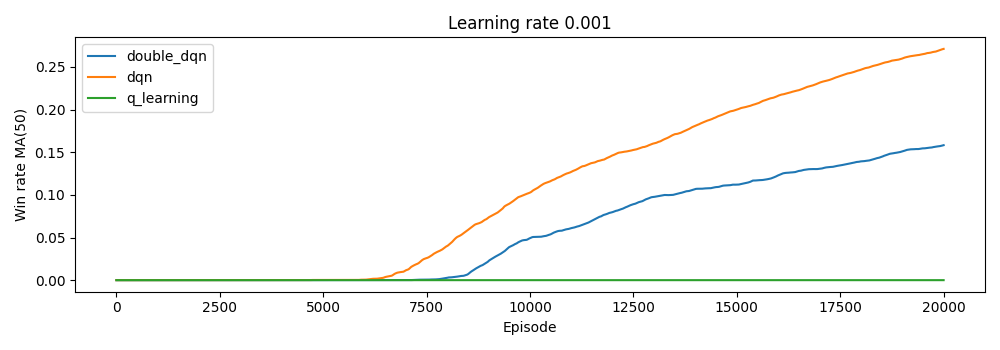
\includegraphics[width=0.85\textwidth]{image/win_rate_001.png}
    \caption{Tỷ lệ thắng tích lũy trong quá trình training, được làm mượt bằng trung bình trượt 50 episode, với các mức learning rate lần lượt từ trên xuống dưới là $0{,}0001$, $0{,}0005$ và $0{,}001$.}
    \label{fig:winrate-comparison}
\end{figure}

Win rate trên đồ thị là tỷ lệ thắng tích lũy từ đầu quá trình training. Trong khi đó, \tabref{tab:winrate-progress} sử dụng win rate của 20 episode evaluation độc lập tại từng checkpoint. Ở cả hai trường hợp, một episode được tính là thắng khi tác tử thu thập đủ 62 food.

\begin{table}[H]
    \centering
    \renewcommand{\arraystretch}{1.2}
    \small
    \begin{tabular}{cccccc}
        \toprule
        \textbf{Cấu hình} & \makecell{\textbf{10.000}\\\textbf{episode}} & \makecell{\textbf{11.000}\\\textbf{episode}} & \makecell{\textbf{12.000}\\\textbf{episode}} & \makecell{\textbf{15.000}\\\textbf{episode}} & \makecell{\textbf{20.000}\\\textbf{episode}} \\
        \midrule
        Double DQN ($\mathrm{LR}=0{,}0001$) & $80\%$ & $95\%$ & $85\%$ & $80\%$ & $95\%$ \\
        DQN ($\mathrm{LR}=0{,}0005$) & $45\%$ & $0\%$ & $100\%$ & $100\%$ & $95\%$ \\
        Q-Learning ($\mathrm{LR}=0{,}001$) & $0\%$ & $0\%$ & $0\%$ & $0\%$ & $0\%$ \\
        \bottomrule
    \end{tabular}
    \caption{Win rate tại các mốc đánh giá.}
    \label{tab:winrate-progress}
\end{table}

Win rate cho thấy thời điểm policy chuyển từ gần hoàn thành sang hoàn thành thực sự. DQN có win rate $45\%$ tại episode 10.000, thấp hơn mức $80\%$ của Double DQN. Sau đó, DQN biến động mạnh và đạt $100\%$ tại episode 12.000, đồng thời duy trì mức này ở episode 15.000.

Dao động lớn nhất xuất hiện ở DQN tại episode 11.000. Reward giảm từ $982{,}988$ xuống $138{,}031$, completion rate giảm từ $91{,}21\%$ xuống $38{,}31\%$ và cả 20 episode đều kết thúc do bị bắt. Ngay tại episode 12.000, policy lại thắng 20/20 episode với completion rate $100\%$. Sự suy giảm đồng thời trên nhiều metric cho thấy đây là một checkpoint có hiệu năng thấp, không chỉ là biến động riêng của win rate. Dù vậy, một training seed chưa đủ để quy nguyên nhân cho catastrophic forgetting. Double DQN cũng dao động từ $95\%$ ở episode 11.000 xuống $80\%$ ở episode 15.000, nhưng không xuất hiện mức sụt về $0\%$ như DQN.

\subsubsection{Steps}

\begin{figure}[H]
    \centering
    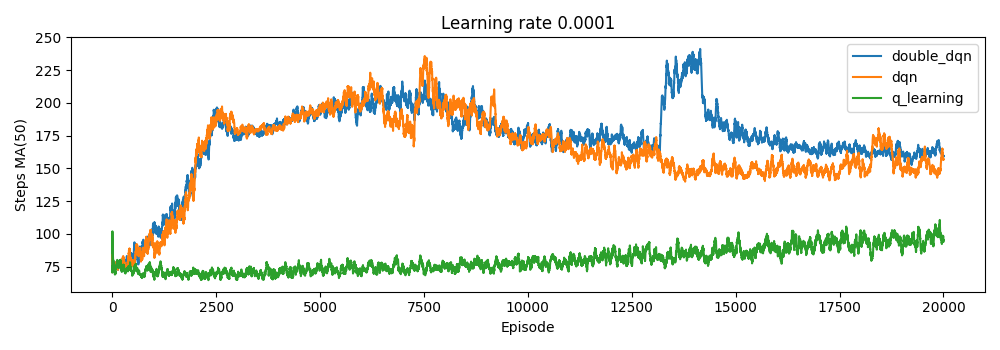
\includegraphics[width=0.85\textwidth]{image/steps_0001.png}
    \par\vspace{0.3cm}
    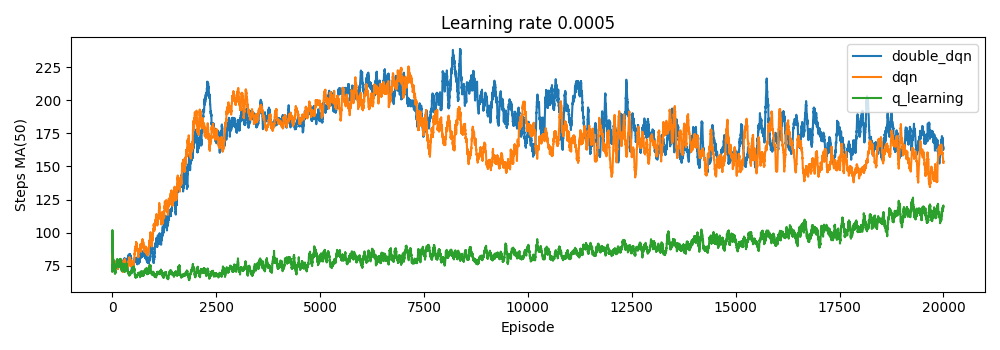
\includegraphics[width=0.85\textwidth]{image/steps_0005.png}
    \par\vspace{0.3cm}
    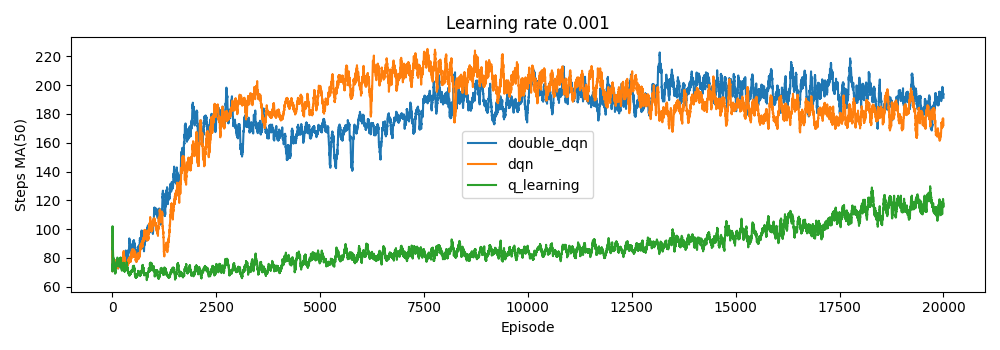
\includegraphics[width=0.85\textwidth]{image/steps_001.png}
    \caption{Số bước trong quá trình training, được làm mượt bằng trung bình trượt 50 episode, với các mức learning rate lần lượt từ trên xuống dưới là $0{,}0001$, $0{,}0005$ và $0{,}001$.}
    \label{fig:steps-comparison}
\end{figure}

Số bước trung bình phản ánh độ dài của episode trước khi tác tử thắng, mất mạng cuối cùng hoặc đạt giới hạn bước. Vì episode thất bại sớm cũng có thể có ít bước, chỉ số này phải được đọc cùng win rate và completion rate. \tabref{tab:steps-progress} trình bày số bước trung bình từ các lần evaluation tại năm mốc training.

\begin{table}[H]
    \centering
    \renewcommand{\arraystretch}{1.2}
    \small
    \begin{tabular}{cccccc}
        \toprule
        \textbf{Cấu hình} & \makecell{\textbf{1.000}\\\textbf{episode}} & \makecell{\textbf{5.000}\\\textbf{episode}} & \makecell{\textbf{10.000}\\\textbf{episode}} & \makecell{\textbf{15.000}\\\textbf{episode}} & \makecell{\textbf{20.000}\\\textbf{episode}} \\
        \midrule
        Double DQN ($\mathrm{LR}=0{,}0001$) & $219{,}00$ & $235{,}60$ & $163{,}25$ & $176{,}35$ & $148{,}30$ \\
        DQN ($\mathrm{LR}=0{,}0005$) & $210{,}90$ & $229{,}95$ & $177{,}85$ & $134{,}25$ & $138{,}90$ \\
        Q-Learning ($\mathrm{LR}=0{,}001$) & $66{,}00$ & $85{,}20$ & $89{,}05$ & $99{,}60$ & $134{,}40$ \\
        \bottomrule
    \end{tabular}
    \caption{Số bước trung bình tại các mốc đánh giá.}
    \label{tab:steps-progress}
\end{table}

Số bước chỉ có ý nghĩa khi được đối chiếu với kết quả kết thúc episode. Tại episode 5.000, DQN và Double DQN cần trung bình khoảng 230 bước, đạt completion rate trên $95\%$ nhưng gần như không thắng. Các episode dài ở giai đoạn này cho thấy tác tử đã tồn tại đủ lâu để thu thập phần lớn food, nhưng chưa hoàn thành được phần cuối của bản đồ. Đến episode 15.000, DQN thắng 20/20 episode và số bước giảm còn $134{,}25$. Việc số bước giảm đồng thời với win rate tăng cho thấy policy đã hoàn thành episode hiệu quả hơn, thay vì kết thúc sớm do bị bắt.

Tại lần evaluation cuối, DQN và Double DQN cùng thắng 19/20 episode, với số bước trung bình lần lượt là $138{,}90$ và $148{,}30$. DQN sử dụng ít bước hơn trong cùng điều kiện hoàn thành gần tương đương, nhưng dữ liệu chưa đủ để khẳng định đây là đường đi ngắn nhất. Đối với Q-Learning, số bước tăng từ $66{,}00$ lên $134{,}40$ cùng với completion rate tăng từ $8{,}39\%$ lên $46{,}29\%$. Vì tất cả episode cuối vẫn kết thúc do bị bắt, xu hướng này phản ánh khả năng tồn tại và thu thập food được cải thiện, không phải hiệu quả hoàn thành.

\subsubsection{Loss}

\begin{figure}[H]
    \centering
    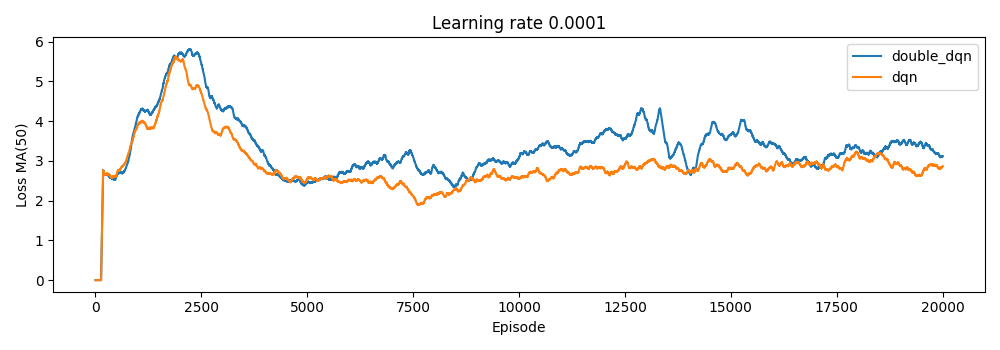
\includegraphics[width=0.85\textwidth]{image/loss_0001.png}
    \par\vspace{0.3cm}
    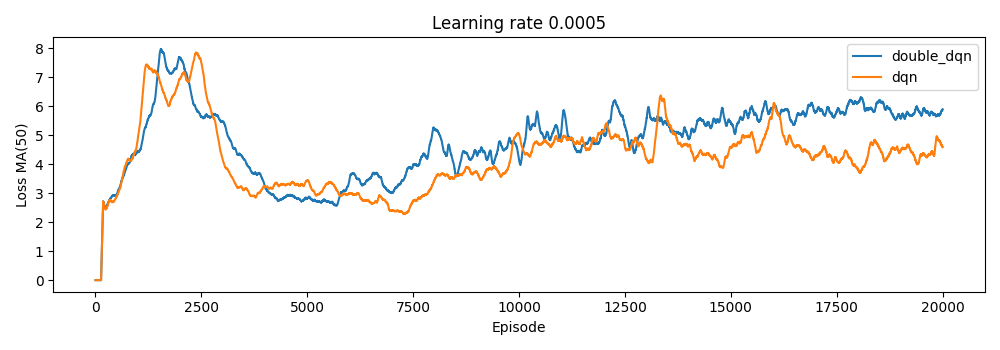
\includegraphics[width=0.85\textwidth]{image/loss_0005.png}
    \par\vspace{0.3cm}
    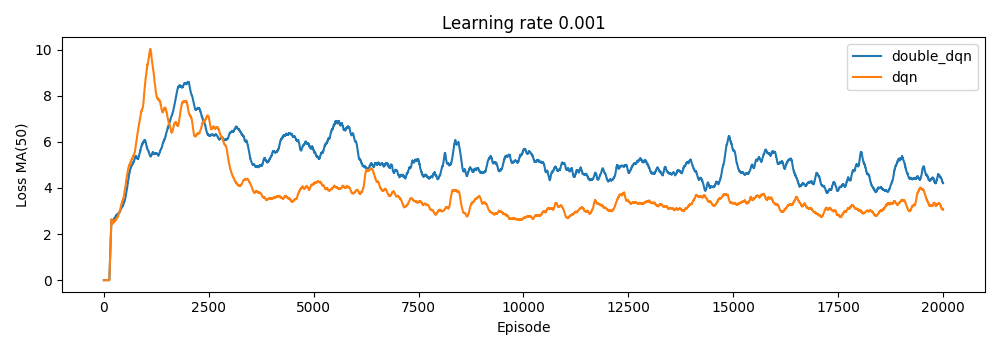
\includegraphics[width=0.85\textwidth]{image/loss_001.png}
    \caption{Smooth L1 Loss trong quá trình training, được làm mượt bằng trung bình trượt 50 episode, với các mức learning rate lần lượt từ trên xuống dưới là $0{,}0001$, $0{,}0005$ và $0{,}001$.}
    \label{fig:loss-comparison}
\end{figure}

Smooth L1 Loss chỉ áp dụng cho DQN và Double DQN. Chỉ số này là trung bình loss của các lần cập nhật mạng trong một episode training. \tabref{tab:loss-progress} tổng hợp giá trị tại một số mốc của hai cấu hình có win rate cuối cao nhất.

\begin{table}[H]
    \centering
    \renewcommand{\arraystretch}{1.2}
    \small
    \begin{tabular}{ccccc}
        \toprule
        \textbf{Cấu hình} & \makecell{\textbf{5.000}\\\textbf{episode}} & \makecell{\textbf{10.000}\\\textbf{episode}} & \makecell{\textbf{15.000}\\\textbf{episode}} & \makecell{\textbf{20.000}\\\textbf{episode}} \\
        \midrule
        DQN ($\mathrm{LR}=0{,}0005$) & $3{,}42$ & $4{,}74$ & $4{,}60$ & $4{,}78$ \\
        Double DQN ($\mathrm{LR}=0{,}0001$) & $2{,}43$ & $3{,}28$ & $3{,}67$ & $2{,}86$ \\
        \bottomrule
    \end{tabular}
    \caption{Loss trung bình trong episode tại các mốc training.}
    \label{tab:loss-progress}
\end{table}

Trước khi replay buffer tích lũy đủ 10.000 environment step, loss bằng $0$ vì online network chưa được cập nhật. Khi quá trình tối ưu bắt đầu, loss tăng nhanh rồi chuyển sang trạng thái dao động. Loss không giảm đều về $0$ do target thay đổi theo chính policy đang học và phân phối mẫu trong replay buffer cũng liên tục biến đổi.

DQN với $\mathrm{LR}=0{,}0005$ có loss $4{,}60$ tại episode 15.000 và $4{,}78$ tại episode 20.000, dù win rate tương ứng là $100\%$ và $95\%$. Điều này cho thấy loss không cần đạt giá trị nhỏ nhất để policy có hiệu năng cao. Double DQN với $\mathrm{LR}=0{,}0001$ có loss thấp hơn tại các mốc được thống kê, nhưng hai cấu hình sử dụng learning rate khác nhau nên không thể quy toàn bộ chênh lệch cho cơ chế Double DQN. Loss vì thế chỉ được dùng để theo dõi quá trình cập nhật mạng, còn chất lượng policy phải được đánh giá bằng reward, completion rate và win rate.

\subsection{Ảnh hưởng của learning rate}

Learning rate ($\alpha$) ảnh hưởng khác nhau đến từng thuật toán. \tabref{tab:lr-trend} sắp xếp kết quả theo thứ tự $\mathrm{LR}=0{,}0001 \rightarrow 0{,}0005 \rightarrow 0{,}001$ để thể hiện trực tiếp xu hướng của từng chỉ số.

\begin{table}[H]
    \centering
    \renewcommand{\arraystretch}{1.2}
    \setlength{\tabcolsep}{4pt}
    \footnotesize
    \begin{tabular}{lccc}
        \toprule
        \textbf{Thuật toán} & \textbf{Số thắng/20} & \textbf{Completion rate (\%)} & \textbf{Steps} \\
        \midrule
        Q-Learning & $0 \rightarrow 0 \rightarrow 0$ & $26{,}29 \rightarrow 42{,}66 \rightarrow 46{,}29$ & $99{,}25 \rightarrow 124{,}05 \rightarrow 134{,}40$ \\
        DQN & $15 \rightarrow 19 \rightarrow 15$ & $98{,}55 \rightarrow 99{,}84 \rightarrow 98{,}71$ & $157{,}85 \rightarrow 138{,}90 \rightarrow 161{,}85$ \\
        Double DQN & $19 \rightarrow 17 \rightarrow 13$ & $99{,}76 \rightarrow 99{,}27 \rightarrow 99{,}27$ & $148{,}30 \rightarrow 153{,}60 \rightarrow 211{,}65$ \\
        \bottomrule
    \end{tabular}
    \caption{Xu hướng kết quả khi learning rate tăng từ $0{,}0001$ lên $0{,}001$ \cite{DRLPacmanGitHub}.}
    \label{tab:lr-trend}
\end{table}

\noindent\textbf{Q-Learning.} Trong ba cấu hình đã chạy, learning rate tăng đi kèm với reward, completion rate và số bước trung bình cùng tăng. $\mathrm{LR}=0{,}001$ đạt reward $165{,}472$ và completion rate $46{,}29\%$, cao hơn hai mức còn lại, nhưng cả 20 episode evaluation vẫn kết thúc do bị bắt. Như vậy, learning rate lớn hơn giúp policy đi xa hơn và thu thập nhiều food hơn trong miền đã khảo sát, song chưa làm thay đổi kết quả cuối cùng là win rate $0\%$. Do learning rate lớn nhất mới chỉ bằng $0{,}001$, thí nghiệm chưa xác định được mức phù hợp nhất cho cập nhật Q-table.

\noindent\textbf{DQN.} Hai mức còn lại là $\mathrm{LR}=0{,}0001$ và $\mathrm{LR}=0{,}001$ đều thắng 15/20 episode, trong khi $\mathrm{LR}=0{,}0005$ thắng 19/20 episode. Cấu hình này cũng có completion rate cao nhất là $99{,}84\%$ và số bước thấp nhất là $138{,}90$. Cả ba chỉ số đều cho thấy $\mathrm{LR}=0{,}0005$ là cấu hình cân bằng nhất của DQN trong miền đã khảo sát. Tuy nhiên, ba điểm dữ liệu và một training seed chưa đủ để kết luận quan hệ giữa learning rate và hiệu năng có dạng cụ thể.

\noindent\textbf{Double DQN.} Khi learning rate tăng, số episode thắng giảm lần lượt từ 19 xuống 17 và 13, trong khi số episode bị bắt tăng từ 1 lên 3 và 7. Completion rate của cả ba cấu hình vẫn trên $99\%$, cho thấy các episode thất bại thường kết thúc khi tác tử đã thu thập gần hết food. Đồng thời, reward tăng từ $1247{,}154$ lên $1553{,}422$ và số bước tăng từ $148{,}30$ lên $211{,}65$. Vì log không tách reward theo sự kiện, chưa thể xác định nguồn reward tăng thêm. Tuy nhiên, kết quả đủ cho thấy $\mathrm{LR}=0{,}001$ tạo ra policy có reward cao nhưng mất nhiều bước hơn và bị bắt thường xuyên hơn. Xét mục tiêu hoàn thành màn chơi, $\mathrm{LR}=0{,}0001$ là cấu hình phù hợp nhất của Double DQN trong ba mức đã thử.

\subsection{Tổng hợp kết quả thực nghiệm}

Tại episode 20.000, \tabref{tab:representative-comparison} đối chiếu cấu hình có win rate cao nhất của từng thuật toán. Cột kết quả lần lượt ghi số episode thắng, bị bắt và timeout trong 20 episode evaluation.

\begin{table}[H]
    \centering
    \renewcommand{\arraystretch}{1.2}
    \setlength{\tabcolsep}{5pt}
    \footnotesize
    \begin{tabular}{lcccc}
        \toprule
        \textbf{Cấu hình} & \makecell{\textbf{Thắng/Bị bắt}\\\textbf{/Timeout}} & \textbf{Reward} & \makecell{\textbf{Completion}\\\textbf{rate}} & \textbf{Steps} \\
        \midrule
        Q-Learning ($\mathrm{LR}=0{,}001$) & $0/20/0$ & $165{,}472$ & $46{,}29\%$ & $134{,}40$ \\
        DQN ($\mathrm{LR}=0{,}0005$) & $19/1/0$ & $1254{,}443$ & $99{,}84\%$ & $138{,}90$ \\
        Double DQN ($\mathrm{LR}=0{,}0001$) & $19/1/0$ & $1247{,}154$ & $99{,}76\%$ & $148{,}30$ \\
        \bottomrule
    \end{tabular}
    \caption{Đối chiếu ba cấu hình đại diện tại episode 20.000 \cite{DRLPacmanGitHub}.}
    \label{tab:representative-comparison}
\end{table}

Q-Learning không thắng episode nào và cả 20 episode đều kết thúc do bị bắt. Completion rate $46{,}29\%$ cho thấy tác tử đã học được cách thu thập một phần food, nhưng chưa học được policy hoàn thành bản đồ.

DQN và Double DQN có cùng số episode thắng và cùng số lần bị bắt. DQN có completion rate cao hơn $0{,}08$ điểm phần trăm và sử dụng ít hơn trung bình $9{,}40$ bước. Chênh lệch này ủng hộ việc chọn DQN $\mathrm{LR}=0{,}0005$ khi ưu tiên số bước, nhưng một training seed chưa đủ để khẳng định DQN tốt hơn Double DQN về tổng quát.

Reward cũng không thể được dùng làm tiêu chí duy nhất. Double DQN với $\mathrm{LR}=0{,}001$ đạt reward cao nhất là $1553{,}422$, nhưng chỉ thắng 13/20 episode, bị bắt 7 lần và cần trung bình $211{,}65$ bước. Vì vậy, DQN $\mathrm{LR}=0{,}0005$ và Double DQN $\mathrm{LR}=0{,}0001$ là hai cấu hình cân bằng nhất khi xét đồng thời win rate, completion rate và số bước.

\subsection{Hạn chế của thực nghiệm}

Mỗi cấu hình chỉ được training một lần với seed 42. Vì chưa có các lần chạy độc lập, báo cáo chưa xác định được độ biến động giữa các seed, độ lệch chuẩn hoặc khoảng tin cậy. Những chênh lệch nhỏ giữa các cấu hình vì thế cần được diễn giải thận trọng.

Mỗi lần evaluation gồm 20 episode với seed 10042 nên win rate thay đổi theo bước $5\%$. Seed cố định tạo điều kiện so sánh nhất quán, nhưng chưa phản ánh hiệu năng trên nhiều chuỗi ngẫu nhiên. Log cũng chỉ lưu reward tổng, chưa tách đóng góp của các sự kiện như ăn ghost, bonus fruit hoặc va tường.

Q-Learning dùng tuple state 17 giá trị, còn DQN và Double DQN dùng vector 92 chiều với nhiều thông tin bổ sung. Chênh lệch kết quả do đó chịu ảnh hưởng đồng thời của thuật toán và cách biểu diễn state. Thiết kế hiện tại chưa tách riêng hai yếu tố này.

Ba learning rate được dùng chung cho cả ba thuật toán, dù chúng tác động lên Q-table và optimizer Adam theo cách khác nhau. Miền khảo sát chưa chắc chứa cấu hình tốt nhất cho từng phương pháp. Kết quả chỉ cho phép so sánh ba mức đã chọn.

Thực nghiệm mới được thực hiện trên bản đồ \texttt{medium}, với ba ma, ba mạng sống và một thiết kế reward cố định. Khả năng khái quát sang điều kiện khác cần được kiểm chứng bằng thí nghiệm bổ sung.

\subsection{Hướng dẫn chạy demo}

Demo cho phép lựa chọn một trong chín final model đã huấn luyện của Q-Learning, DQN và Double DQN. Trong quá trình chạy, tác tử chỉ sử dụng policy đã lưu để lựa chọn action. Q-table và tham số mạng không được cập nhật. Các lệnh dưới đây được thực hiện trong PowerShell tại thư mục gốc của repository \cite{DRLPacmanGitHub}.

\begin{enumerate}
    \item \textbf{Chuẩn bị môi trường.} Bước này chỉ cần thực hiện trong lần chạy đầu tiên.

    {\small
    \begin{verbatim}
conda create -n pacman python=3.10 -y
conda activate pacman
pip install -r requirements.txt
    \end{verbatim}
    }

    \item \textbf{Mở danh sách lựa chọn model.} Chạy lệnh sau để chương trình quét thư mục \texttt{models/final} và hiển thị các model hiện có.

    {\small
    \begin{verbatim}
python -m src.training.watch_finals
    \end{verbatim}
    }

    Mỗi dòng trong danh sách gồm số thứ tự, thuật toán, learning rate và đường dẫn tới final model. Người dùng nhập số tương ứng rồi nhấn \texttt{Enter} để chạy model. Chẳng hạn, nhập \texttt{5} để chọn DQN với $\mathrm{LR}=0{,}0005$, là cấu hình DQN có kết quả cuối tốt nhất trong thực nghiệm. Lựa chọn \texttt{a} dùng để chạy lần lượt toàn bộ model. Giao diện lựa chọn được minh họa trong \figref{fig:demo-model-selection}.

    \begin{figure}[H]
        \centering
        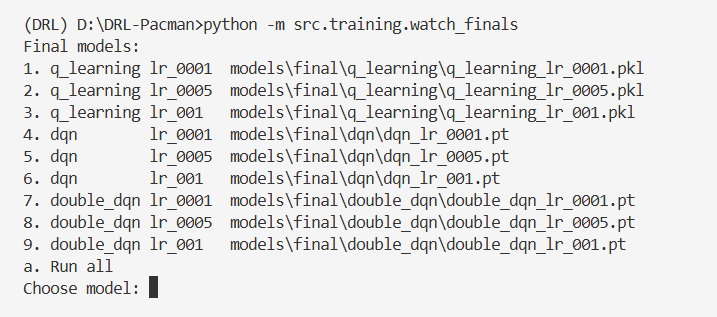
\includegraphics[width=0.82\textwidth]{image/choose_model.png}
        \caption{Danh sách lựa chọn final model khi chạy demo.}
        \label{fig:demo-model-selection}
    \end{figure}

    \item \textbf{Quan sát tác tử.} Sau khi model được chọn, cửa sổ Mini Pacman mở và policy tự động điều khiển Pacman. Phần trên của giao diện hiển thị episode hiện tại, số bước, action vừa chọn và sự kiện trong môi trường. Mặc định, chương trình chạy ba episode với độ trễ 500 ms giữa hai bước.

    Khi Pacman thu thập đủ 62 food, episode kết thúc với thông báo \textit{You Win}. Nếu Pacman mất mạng cuối cùng hoặc chạm giới hạn số bước, giao diện hiển thị \textit{You Lose}. Hai trạng thái kết thúc được thể hiện trong \figref{fig:demo-results}.

    \begin{figure}[H]
        \centering
        \begin{subfigure}[t]{0.39\textwidth}
            \centering
            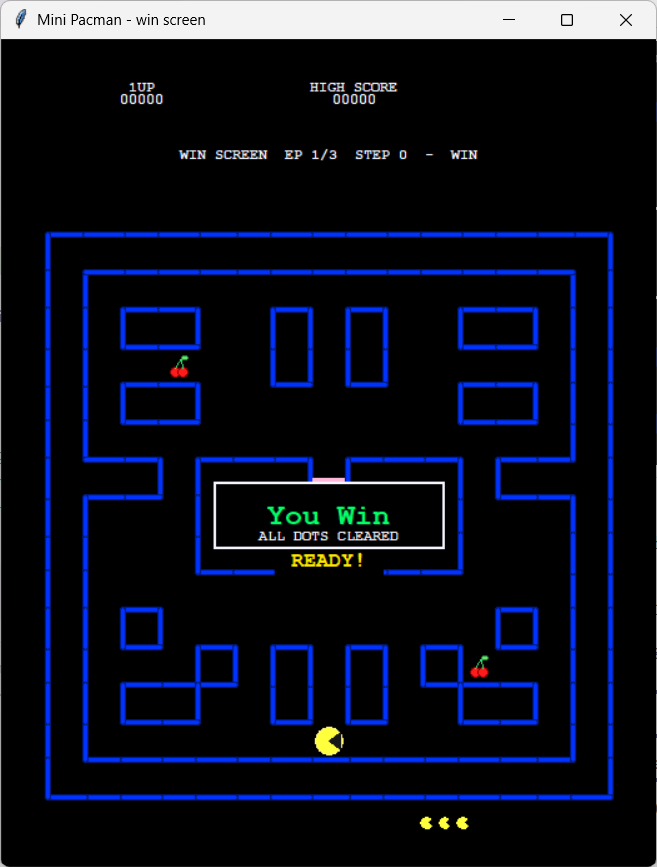
\includegraphics[width=\textwidth]{image/pacman_win.png}
            \caption{Pacman hoàn thành bản đồ.}
            \label{fig:demo-win}
        \end{subfigure}%
        \hspace{0.025\textwidth}%
        \begin{subfigure}[t]{0.39\textwidth}
            \centering
            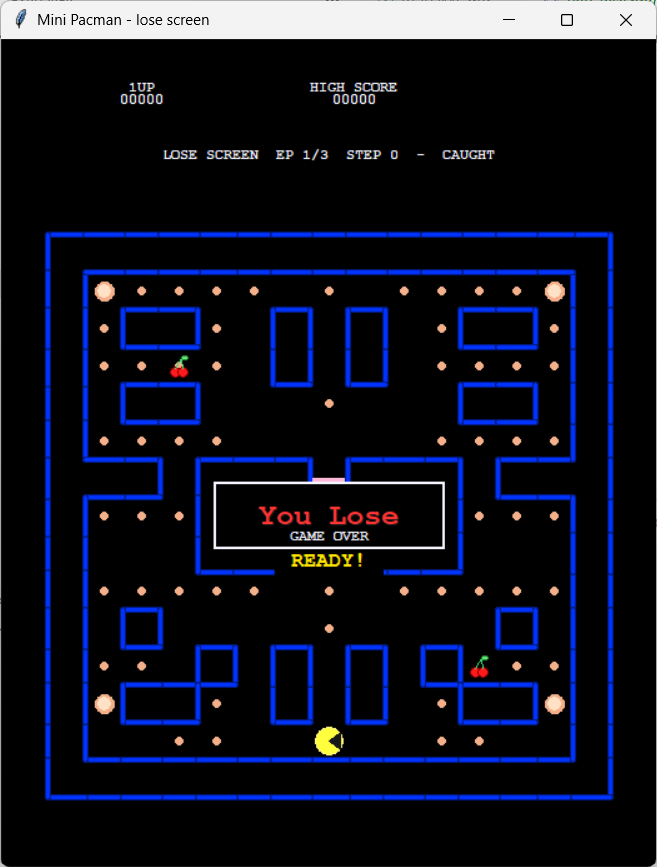
\includegraphics[width=\textwidth]{image/pacman_lose.png}
            \caption{Pacman kết thúc episode do bị bắt.}
            \label{fig:demo-lose}
        \end{subfigure}
        \caption{Hai trạng thái kết thúc có thể quan sát trong giao diện demo.}
        \label{fig:demo-results}
    \end{figure}

    \item \textbf{Điều chỉnh hiển thị.} Số episode và tốc độ hiển thị có thể được thay đổi bằng các tham số sau.

    {\small
    \begin{verbatim}
python -m src.training.watch_finals --episodes 5 --delay-ms 150
    \end{verbatim}
    }

    Trong lệnh trên, \texttt{--episodes 5} đặt số episode chạy cho model được chọn, còn \texttt{--delay-ms 150} rút ngắn thời gian chờ giữa hai bước xuống 150 ms. Sau khi nhập lệnh, người dùng vẫn chọn model từ danh sách như ở bước 2.
\end{enumerate}

Người dùng có thể đóng cửa sổ Mini Pacman tại bất kỳ thời điểm nào để kết thúc demo hiện tại.

\clearpage
\section{KẾT LUẬN VÀ HƯỚNG PHÁT TRIỂN}

\subsection{Kết luận}

Đề tài đã xây dựng môi trường Mini Pacman, cài đặt Q-Learning, DQN và Double DQN, sau đó thực hiện chín cấu hình thí nghiệm trên bản đồ \texttt{medium}. Kết quả thu được đáp ứng các mục tiêu nghiên cứu trong phạm vi đã xác định ở Chương 1. Những kết luận chính gồm:

\begin{enumerate}
    \item \textbf{Về hệ thống và quy trình thực nghiệm.} Môi trường mô phỏng đầy đủ các thành phần cần thiết của bài toán gồm Pacman, food, power pellet, bonus fruit, ba ma, số mạng và điều kiện kết thúc episode. Repository tổ chức cấu hình bằng YAML, hỗ trợ lưu checkpoint, tiếp tục training, ghi metrics, lưu final model, vẽ biểu đồ và chạy evaluation độc lập với $\epsilon=0$ \cite{DRLPacmanGitHub}. Nhờ đó, chín cấu hình được thực hiện theo cùng một quy trình và có thể đối chiếu bằng cùng nhóm chỉ số.

    \item \textbf{Về kết quả của ba thuật toán.} \tabref{tab:representative-comparison} cho thấy sự khác biệt rõ ràng giữa ba cấu hình đại diện tại episode 20.000.
    \begin{itemize}
        \item Q-Learning với $\mathrm{LR}=0{,}001$ không thắng episode nào, cả 20 episode đều kết thúc do bị bắt và completion rate đạt $46{,}29\%$. Kết quả cho thấy Q-table đã tạo ra tiến bộ về khả năng thu thập food, nhưng chưa hình thành policy hoàn thành bản đồ trong giới hạn training của đề tài.

        \item DQN với $\mathrm{LR}=0{,}0005$ thắng 19/20 episode, đạt completion rate $99{,}84\%$ và cần trung bình $138{,}90$ bước. Đây là cấu hình DQN cân bằng nhất trong ba learning rate đã thử.

        \item Double DQN với $\mathrm{LR}=0{,}0001$ cũng thắng 19/20 episode, đạt completion rate $99{,}76\%$ và cần trung bình $148{,}30$ bước. Kết quả gần tương đương DQN về khả năng hoàn thành, nhưng số bước trung bình cao hơn $9{,}40$.
    \end{itemize}

    Trong thiết kế hiện tại, hai cấu hình sử dụng Q-network đạt kết quả cao hơn Q-Learning. Tuy nhiên, Q-Learning dùng tuple state 17 giá trị, còn DQN và Double DQN dùng vector 92 chiều. Vì vậy, chênh lệch quan sát được chịu ảnh hưởng đồng thời của thuật toán và cách biểu diễn state, không thể được quy hoàn toàn cho riêng thuật toán.

    \item \textbf{Về learning rate và cách đọc metrics.} \tabref{tab:lr-trend} cho thấy learning rate phù hợp phụ thuộc vào từng phương pháp. DQN đạt kết quả tốt nhất tại mức giữa $\mathrm{LR}=0{,}0005$. Với Double DQN, số episode thắng giảm từ 19 xuống 17 và 13 khi learning rate tăng. Q-Learning cải thiện completion rate khi learning rate tăng trong miền khảo sát, nhưng win rate vẫn bằng $0\%$.

    Reward cần được đọc cùng win rate, completion rate và steps. Double DQN với $\mathrm{LR}=0{,}001$ đạt reward cao nhất là $1553{,}422$, nhưng chỉ thắng 13/20 episode và cần trung bình $211{,}65$ bước. Tương tự, sự suy giảm của DQN tại episode 11.000 xuất hiện đồng thời trên nhiều metrics, nhưng một training seed chưa đủ để xác định nguyên nhân là overestimation bias hay catastrophic forgetting.
\end{enumerate}

Nhìn chung, đề tài đã hoàn thành việc xây dựng môi trường, cài đặt ba thuật toán và tổ chức quy trình so sánh bằng dữ liệu định lượng. Các kết quả chỉ đại diện cho chín cấu hình, một training seed, một evaluation seed và bản đồ \texttt{medium}. Do đó, chúng không được xem là kết luận chung về hiệu quả của các thuật toán trong mọi bài toán học tăng cường.

\subsection{Hướng phát triển}

Các hướng phát triển được đề xuất trực tiếp từ những hạn chế của thiết kế thực nghiệm hiện tại:

\begin{enumerate}
    \item \textbf{Tăng độ tin cậy của kết quả.}
    \begin{itemize}
        \item Training mỗi cấu hình với nhiều seed độc lập, sau đó báo cáo giá trị trung bình, độ lệch chuẩn và khoảng tin cậy.
        \item Tăng số episode evaluation và sử dụng nhiều evaluation seed để giảm ảnh hưởng của một chuỗi ngẫu nhiên cố định.
        \item Khảo sát learning rate riêng cho từng thuật toán thay vì dùng chung ba mức cho cả Q-table và optimizer Adam.
    \end{itemize}

    \item \textbf{Tách ảnh hưởng của thuật toán và biểu diễn state.}
    \begin{itemize}
        \item Xây dựng thí nghiệm ablation để so sánh các thuật toán trên cùng tập đặc trưng đầu vào.
        \item Thử các biến thể state có và không có thông tin về food gần nhất, ma gần nhất, action hợp lệ và action nguy hiểm.
        \item Khi đã có đường cơ sở công bằng, có thể thử đầu vào ảnh kết hợp mạng nơ-ron tích chập để đánh giá khả năng tự trích xuất đặc trưng.
    \end{itemize}

    \item \textbf{Mở rộng metrics và thiết kế reward.}
    \begin{itemize}
        \item Tách reward theo từng sự kiện như ăn food, ăn ghost, lấy bonus fruit, mất mạng và va tường.
        \item Ghi thêm số lần đổi hướng, chọn action nguy hiểm và thời gian ở trạng thái frightened để định lượng hành vi trong demo.
        \item Thử các cấu hình reward khác nhau và đánh giá bằng cả win rate, completion rate lẫn steps thay vì chỉ dựa trên reward tổng.
    \end{itemize}

    \item \textbf{Mở rộng môi trường và thuật toán.}
    \begin{itemize}
        \item Thử nghiệm trên nhiều bản đồ, số lượng ma và mức độ truy đuổi khác nhau để kiểm tra khả năng khái quát của policy.
        \item Nghiên cứu Dueling DQN và Prioritized Experience Replay trên cùng quy trình evaluation hiện tại.
        \item Thử các phương pháp Actor-Critic hoặc Proximal Policy Optimization để mở rộng so sánh ngoài nhóm thuật toán dựa trên giá trị.
    \end{itemize}
\end{enumerate}

\newpage

\renewcommand{\refname}{TÀI LIỆU THAM KHẢO}
\addcontentsline{toc}{section}{TÀI LIỆU THAM KHẢO}

\begin{thebibliography}{99}

\bibitem{SuttonBarto2018}
R. S. Sutton and A. G. Barto,
\href{http://incompleteideas.net/book/the-book-2nd.html}
{\textit{Reinforcement Learning: An Introduction}},
2nd ed.
Cambridge, MA, USA: MIT Press, 2018.

\bibitem{WatkinsDayan1992}
C. J. C. H. Watkins and P. Dayan,
\href{https://doi.org/10.1007/BF00992698}
{``Q-Learning,''}
\textit{Machine Learning},
vol. 8,
no. 3--4,
pp. 279--292,
1992.

\bibitem{Mnih2013}
V. Mnih, K. Kavukcuoglu, D. Silver, A. Graves,
I. Antonoglou, D. Wierstra, and M. Riedmiller,
\href{https://arxiv.org/abs/1312.5602}
{``Playing Atari with Deep Reinforcement Learning,''}
\textit{arXiv preprint arXiv:1312.5602},
2013.

\bibitem{Mnih2015}
V. Mnih, K. Kavukcuoglu, D. Silver, A. A. Rusu, J. Veness,
M. G. Bellemare, A. Graves, M. Riedmiller, A. K. Fidjeland,
G. Ostrovski, S. Petersen, C. Beattie, A. Sadik, I. Antonoglou,
H. King, D. Kumaran, D. Wierstra, S. Legg, and D. Hassabis,
\href{https://doi.org/10.1038/nature14236}
{``Human-Level Control Through Deep Reinforcement Learning,''}
\textit{Nature},
vol. 518,
no. 7540,
pp. 529--533,
2015.

\bibitem{VanHasselt2016}
H. van Hasselt, A. Guez, and D. Silver,
\href{https://doi.org/10.1609/aaai.v30i1.10295}
{``Deep Reinforcement Learning with Double Q-Learning,''}
in \textit{Proceedings of the AAAI Conference on Artificial Intelligence},
vol. 30, no. 1, pp. 2094--2100, 2016.

\bibitem{BerkeleyPacman2024}
University of California, Berkeley,
\href{https://inst.eecs.berkeley.edu/~cs188/}
{``CS 188 Project 3: Reinforcement Learning,''}
Department of Electrical Engineering and Computer Sciences,
Pacman Artificial Intelligence Projects,
2024.

\bibitem{DRLPacmanGitHub}
Đặng Anh Tuyền,
\href{https://github.com/tuyenda2011/DRL-Pacman}
{``DRL-Pacman: Q-Learning, DQN and Double DQN on Mini Pacman,''}
GitHub repository, 2026.

\bibitem{TranDinhTanAICourse}
TS. Trần Đình Tân,
{``Nhập môn trí tuệ nhân tạo,''}
Trường Công nghệ Thông tin Phenikaa.

\end{thebibliography}


\end{document}
